\documentclass[11pt]{article}
\usepackage[utf8]{inputenc}
\usepackage[margin=1in]{geometry}
\usepackage{amsmath,amssymb,amsthm,mathtools}
\usepackage{microtype}
\usepackage{xcolor}
\usepackage{tikz}
\usetikzlibrary{arrows.meta}
\usepackage[colorlinks=true,linkcolor=blue!45!black,citecolor=blue!45!black,urlcolor=blue!45!black]{hyperref}
\pdfinfoomitdate=1
\pdftrailerid{}
\pdfsuppressptexinfo=15
\hypersetup{pdftitle={Two limit cycles for quintic Lienard systems},pdfauthor={OpenAI}}
\numberwithin{equation}{section}
\newtheorem{theorem}{Theorem}[section]
\newtheorem{proposition}[theorem]{Proposition}
\newtheorem{lemma}[theorem]{Lemma}
\newtheorem{corollary}[theorem]{Corollary}
\theoremstyle{remark}
\newtheorem{remark}[theorem]{Remark}
\newcommand{\R}{\mathbb R}
\title{Two limit cycles for quintic Li\'enard systems}
\author{OpenAI}
\date{September 24, 2026}
\begin{document}
\maketitle
\begin{abstract}
Every classical Li\'enard system $\dot x=y-F(x)$, $\dot y=-x$,
with $F$ an arbitrary real polynomial of degree at most five,
has at most two geometrically distinct isolated periodic orbits,
and the bound is attained. This proves the degree-five case of the
Lins Neto--de Melo--Pugh conjecture.
\end{abstract}
\section{Introduction}\label{sec:introduction}

Consider the classical Li\'enard system
\begin{equation}\label{eq:original-system}
 \dot x=y-F(x),\qquad \dot y=-x,
\end{equation}
where $F$ is a real polynomial. A limit cycle is the image of a
nonconstant periodic solution that is isolated among periodic
orbits. We count each such image once, irrespective of its
multiplicity, stability, or hyperbolicity. The periodic orbits of
a center are not limit cycles under this convention.

\begin{theorem}\label{thm:main}
If $\deg F\le5$, the system \eqref{eq:original-system} has at most
two limit cycles in $\R^2$. Some members of this class have two
limit cycles. Thus its exact maximum is two.
\end{theorem}

Here the degree is that of the primitive $F$. The equivalent scalar
equation is
\[
 x''+F'(x)x'+x=0,
\]
so its damping polynomial has degree at most four and its restoring
force is exactly $x$. No parity or coefficient-sign assumption is
imposed on $F$.

The problem is a restricted instance of the second part of
Hilbert's sixteenth problem, concerning the number of limit cycles
of polynomial planar vector fields. Lins, de Melo, and Pugh proposed
the bound $\lfloor(n-1)/2\rfloor$ for
\eqref{eq:original-system} with $\deg F=n\ge1$ \cite{LMP}.
Rychkov proved the two-cycle bound for odd quintic primitives
\cite{Rychkov}. Dumortier, Panazzolo, and Roussarie constructed systems with
four cycles and primitive degree seven \cite{DPR}.
De Maesschalck and Dumortier obtained four cycles already in
degree six \cite{DMD}, and De Maesschalck and Huzak subsequently
constructed at least $n-2$ cycles in every degree $n\ge6$
\cite{DMH}. These counterexamples leave degree five undecided.
Li and Llibre established the unrestricted quartic bound of one
cycle \cite{LiLlibre}. Llibre and Zhang survey this development
and the classical perturbative lower bounds \cite{LlibreZhang}.

In degree five, the distinction between a global bound and a
bound in a limiting regime is essential. Li and Lu proved that
nondegenerate slow--fast cycles have cyclicity at most two
\cite{LiLu}. The Introduction of the August 2026 preprint by
Chen, Li, Zhang, and Zhang distinguishes that result from the
unrestricted polynomial problem and reports the latter as open
\cite{CLZZ}. Hern\'andez Rosales proposes a degree-five four-cycle
example for $x''+\mu f(x)x'+x=0$ in Section~9 of \cite{Rosales},
with $\mu=1/10$ and $f(x)=x^4-10x^2+5$. The proposed system has exactly two
limit cycles. Indeed, the change $x=\sqrt5\,u$ transforms its
scalar equation into
\[
 u''+\frac12(5u^4-10u^2+1)u'+u=0.
\]
This is Odani's Example~3 with parameters $\widehat\mu=1/2$ and
$v=10/3>\sqrt5$, for which exactly two periodic solutions are
proved \cite{Odani}. The discrepancy in the proposed amplitude
calculation is that periodicity requires
$\int_0^T f(x)\dot x^2\,dt=0$. Substituting
$x(t)\approx2X\cos t$ gives $2X^4-10X^2+5=0$, the same equation
used for the second proposed pair. Its roots are
$X^2=(5\pm\sqrt{15})/2$, not $1$ and $4$. Thus these two
leading-order calculations do not yield four distinct cycles.

Two-cycle examples are classical. Besides the perturbative
constructions associated with the conjecture \cite{LMP,LlibreZhang},
rigorous transversal-region methods have been applied to Rychkov's
family by Gasull, Giacomini, and Grau \cite{GGG}.
Section~\ref{sec:sharpness} supplies a direct lower-bound proof,
so the exact maximum follows within this article.

\paragraph{Method.}
The even coefficients prevent reduction to the odd quintic family,
and a small-amplitude calculation cannot by itself bound distant
cycles. Our comparison keeps the two half-orbits separate and
uses coordinates available at every transverse amplitude.
On each half-plane, $u=x^2/2$ transforms an orbit into an arch
satisfying $u_y=\phi(u)-y$, where
$\phi(u)=F(\sqrt{2u})$ or $F(-\sqrt{2u})$.
The even coefficients give the same quadratic part in both profiles,
whereas the odd coefficients change sign. This common part suggests
using quadratic profiles as a comparison family.
At a fixed base height $h$, let $y_<,y_>$ be its endpoints and set
$r=(y_>-y_<)/2$ and $M=(y_>+y_<)/2-\phi(h)$.
The first technical step is a global interpolation theorem:
every admissible pair $(M,M_r)$ has a unique fit by a profile
$\lambda(u-h)+\kappa(u-h)^2/2$. Both its range and its
nonvanishing Jacobian are proved in Theorem~\ref{thm:quadratic-fit};
the fit is available throughout $r>0$, $|M|<r$, and $|M_r|<1$.

The fitted slope and curvature evolve according to the two
transport equations of Lemma~\ref{lem:fit-transport}. Their
coefficients are derivatives of the quadratic midpoint function.
The central model estimate, Theorem~\ref{thm:model-inequality},
controls how one of these coefficients changes with width while
the model parameters are held fixed. Its proof combines endpoint
variation, a Riccati linearization, and a Schwarzian identity for
the endpoint correspondence. The solution-ratio identity and chain
rule are classical projective identities; Ovsienko and Tabachnikov
give a concise account \cite{OT}. Schwarzian derivatives have also
been used for cycle bounds through return maps, including the
discontinuous systems studied by Coll, Gasull, and Prohens
\cite{CGP}. Here the map pairs the two endpoints of a quadratic
arc, and the model estimate concerns that correspondence.

Transporting the fitted parameters along an arch then turns
conditions on $\phi'''$ and on $(\phi'-d)/u$, for a fixed real
constant $d$, into monotonicity and separation statements for the
fitted curvature and slope intercept. Propositions
\ref{prop:third-derivative} and~\ref{prop:intercept} formulate these
comparisons for general smooth profiles, independently of the
polynomial application.

For the original system, periodic orbits are zeros of the
difference between the two height-zero midpoint functions on
one common width interval. The quintic coefficient structure
provides a complete sign partition. In the only case allowing two
cycles, a positive integrating factor makes the derivative of
the matching function have the sign of a nondecreasing function.
This bounds isolated zeros even when zeros are multiple or occur
in intervals. The proof therefore counts degenerate cycles
directly; it does not remove them by a generic perturbation.

Section~\ref{sec:arcs} establishes the arc coordinates and the
global matching interpretation. Section~\ref{sec:fitting} proves the global quadratic fit and its
transport law. Section~\ref{sec:model} establishes the model
inequality, and Section~\ref{sec:transport} derives the shape
comparisons for general profiles. Section~\ref{sec:application} proves the upper bound in
Theorem~\ref{thm:main}, and Section~\ref{sec:sharpness} proves
sharpness.

\section{Arc coordinates and periodic-orbit matching}\label{sec:arcs}

We first study a general profile
\(\phi\in C^\infty((0,\infty))\) and the scalar equation
\begin{equation}\label{eq:arc-ode}
  \frac{du}{dy}=\phi(u)-y.
\end{equation}
Here \(y\) is an endpoint coordinate, rather than physical time.
For each \(t>0\), let \(u(y;t)\) be the solution through
\[
  u(\phi(t);t)=t.
\]
The parameter \(t\) will be the peak height. At a lower height \(h\), the
two endpoint values of \(y\) determine a half-width \(r\) and a midpoint
\(M\), measured relative to \(\phi(h)\).

Figure~\ref{fig:arc-coordinates} illustrates these coordinates.
Our first task is to show that width parametrizes every positive-height
arc. We then continue the transverse arcs to height zero, where
matching the two endpoint pairs counts the periodic orbits.

\subsection{Global endpoint data and their transport}

\begin{lemma}[Global arc coordinates]\label{lem:arc-data}
For every \(0<h<t\), the solution through
\((y,u)=(\phi(t),t)\) has exactly two intersections with \(u=h\).
They are transverse and satisfy
\[
  y_<(h,t)<\phi(h)<y_>(h,t).
\]
The part of the solution between them has a unique maximum \(u=t\).
Set
\begin{equation}\label{eq:arc-endpoint-data}
  r(h,t)=\frac{y_>(h,t)-y_<(h,t)}2,\qquad
  M=\frac{y_>(h,t)+y_<(h,t)}2-\phi(h).
\end{equation}
At fixed \(h\), the lower endpoint decreases strictly with \(t\), the
upper endpoint increases strictly, and both derivatives are nonzero.
The map \(t\mapsto r(h,t)\) is a smooth increasing bijection from
\((h,\infty)\) onto \((0,\infty)\).

Consequently \(M\) is a smooth function of \((h,r)\in(0,\infty)^2\).
Writing \(v=M_r\), one has
\begin{equation}\label{eq:arc-strict-data}
  |M(h,r)|<r,\qquad |v(h,r)|<1,\qquad
  r^2\ge 2(t-h).
\end{equation}
For a fixed width, the corresponding base height is strictly increasing
with peak height: \(\partial h/\partial t>0\).

If \(\phi\) is smooth on the whole real line, the same conclusions hold
for arbitrary real \(h<t\). In that case, at each fixed peak \(t\), letting
\(h\) decrease from \(t\) to \(-\infty\) parametrizes the full range
\(0<r<\infty\).
\end{lemma}

\begin{proof}
Differentiating Equation~\eqref{eq:arc-ode} gives
\[
  u_{yy}=\phi'(u)u_y-1.
\]
Thus every critical point in the profile domain is a nondegenerate
maximum, with \(u_{yy}=-1\). On either side of the prescribed peak the
height therefore decreases strictly as one moves away from it, until
the level \(h\) is reached. A second critical point on either branch
would require a minimum between two maxima, which is impossible.

These intersections occur at finite \(y\). Indeed, while a branch remains
in \([h,t]\), the profile is bounded there. For sufficiently large
positive \(y\), Equation~\eqref{eq:arc-ode} gives \(u_y<-1\); for
sufficiently large negative \(y\), it gives \(u_y>1\). In the respective
outward directions these inequalities force the branch to reach \(h\).
There is also no finite-\(y\) failure of continuation while \(u\) stays
in the compact interval \([h,t]\). The strict derivative signs at the
intersections give the displayed endpoint inequalities.

All the endpoints depend smoothly on \((h,t)\), by smooth dependence
of the differential equation and transversality; see, for example,
\cite[Sections~2.2--2.3]{Perko} for the standard differential-equation
facts. To find their peak
derivatives, let \(\xi(y;t)=\partial_t u(y;t)\), with \(y\) held fixed.
Differentiating the moving initial condition gives
\(\xi(\phi(t);t)=1\), because \(u_y=0\) at the peak. Moreover,
\[
  \xi_y=\phi'(u)\xi,
\]
so \(\xi>0\) throughout the arc. Differentiating the endpoint equations
now gives
\[
  (y_<)_t=-\frac{\xi(y_<;t)}{r-M}<0,\qquad
  (y_>)_t=\frac{\xi(y_>;t)}{r+M}>0.
\]
In particular \(r_t>0\). After changing from \(t\) to \(r\),
\[
  v=\frac{(y_>)_t+(y_<)_t}{(y_>)_t-(y_<)_t}\in(-1,1).
\]
The other strict inequality, \(|M|<r\), follows directly from the
endpoint inequalities.

At fixed \(t\), differentiation with respect to \(h\) gives
\[
  (y_<)_h=\frac1{r-M},\qquad
  (y_>)_h=-\frac1{r+M}.
\]
Hence
\begin{equation}\label{eq:arc-width-height}
  \left.\frac{dr}{dh}\right|_t=-\frac{r}{r^2-M^2},\qquad
  \left.\frac{dM}{dh}\right|_t
       =\frac{M}{r^2-M^2}-\phi'(h).
\end{equation}
The first identity implies \(d(r^2)/dh\le-2\).
The nondegenerate maximum gives \(r\to0\) as \(t\downarrow h\), or as
\(h\uparrow t\) with the peak fixed. Integrating the inequality yields
\(r^2\ge2(t-h)\). At fixed \(h\), it follows that \(r\to\infty\) as
\(t\to\infty\). This proves the asserted bijection and its smooth
inverse. Also, at fixed width,
\[
  \left.\frac{\partial h}{\partial t}\right|_r
    =-\frac{r_t}{r_h}>0.
\]
The same proof applies to any compact interval \([h,t]\) in the domain
of a smooth profile. For a profile on the whole real line, the bound
\(r^2\ge2(t-h)\) also proves the last assertion as \(h\to-\infty\).
\end{proof}

\begin{figure}[tb]
\centering
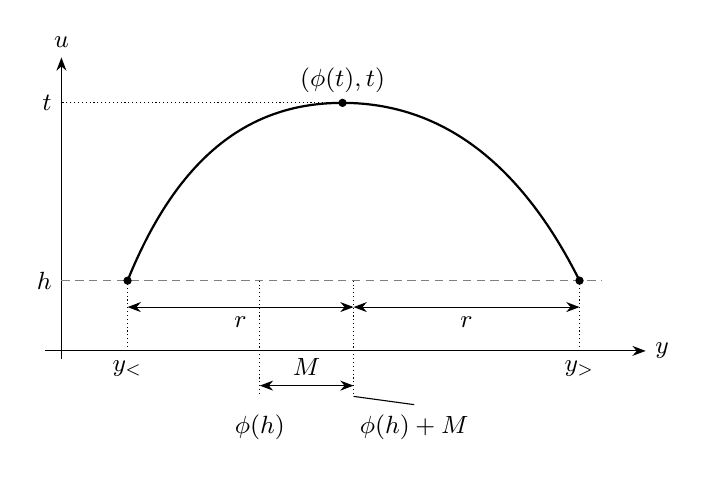
\begin{tikzpicture}[x=1.4cm,y=1.05cm,>=Stealth,font=\small]
  \draw[->] (-2.4,0)--(3.05,0) node[right] {$y$};
  \draw[->] (-2.25,-.1)--(-2.25,3.55) node[above] {$u$};
  \draw[densely dashed,gray] (-2.25,.85)--(2.65,.85);
  \node[left] at (-2.25,.85) {$h$};
  \draw[thick] (-1.65,.85) .. controls (-1.15,2.50) and (-.45,3.0) .. (.30,3.0)
               .. controls (1.08,3.0) and (1.85,2.45) .. (2.45,.85);
  \fill (-1.65,.85) circle (1.5pt);
  \fill (2.45,.85) circle (1.5pt);
  \fill (.30,3.0) circle (1.5pt);
  \draw[densely dotted] (.30,3.0)--(-2.25,3.0);
  \node[left] at (-2.25,3.0) {$t$};
  \node[above] at (.30,3.0) {$(\phi(t),t)$};
  \draw[densely dotted] (-1.65,0)--(-1.65,.85);
  \draw[densely dotted] (2.45,0)--(2.45,.85);
  \node[below] at (-1.65,0) {$y_<$};
  \node[below] at (2.45,0) {$y_>$};
  \draw[densely dotted] (.4,.85)--(.4,-.55);
  \draw[<->] (-1.65,.53)--(.4,.53) node[midway,below] {$r$};
  \draw[<->] (.4,.53)--(2.45,.53) node[midway,below] {$r$};
  \draw[densely dotted] (-.45,.85)--(-.45,-.55);
  \node[below] at (-.45,-.65) {$\phi(h)$};
  \node[below] at (.95,-.65) {$\phi(h)+M$};
  \draw[thin] (.4,-.55)--(.95,-.65);
  \draw[<->] (-.45,-.42)--(.4,-.42) node[midway,above] {$M$};
\end{tikzpicture}
\caption{An arc at base height $h$ and peak height $t$, drawn
schematically with $M>0$. Its endpoint half-width is $r$; its midpoint
is measured relative to $\phi(h)$. Both endpoints move outwards as
the peak rises, giving $|M_r|<1$. The two physical half-orbits form
a periodic orbit precisely when their height-zero endpoint pairs
agree, as proved in Proposition~\ref{prop:cycle-matching}.}
\label{fig:arc-coordinates}
\end{figure}


Put
\[
  k(h)=\phi'(h),\qquad q=r^2-M^2,\qquad
  \alpha=\frac rq,\qquad
  D=\partial_h-\alpha\partial_r.
\]
By Equation~\eqref{eq:arc-width-height}, \(D\) differentiates along a
fixed-peak arc as its base height increases. We call these curves in
the \((h,r)\)-plane \emph{characteristics}. Their basic transport
identities are
\begin{equation}\label{eq:arc-transport}
  DM=\frac Mq-k(h),\qquad
  Dv=-\frac{2Mr(1-v^2)}{q^2}.
\end{equation}
For clarity, the second identity includes a commutator term. For any
smooth function \(f(h,r)\),
\[
  D(f_r)=(Df)_r+\alpha_r f_r,\qquad
  \alpha_r=\frac1q-\frac{2r(r-Mv)}{q^2}.
\]
Using the first identity in Equation~\eqref{eq:arc-transport} therefore
gives
\[
  Dv=\frac{2v}{q}
       -\frac{2(M+rv)(r-Mv)}{q^2}
     =-\frac{2Mr(1-v^2)}{q^2},
\]
as claimed. All partial \(r\)-derivatives here are taken at fixed base
height.

Introduce the angles
\[
  \theta=\operatorname{arctanh}(M/r),\qquad
  L=\operatorname{arctanh}(v).
\]
When a characteristic is parametrized by increasing width \(r\), a
prime denotes the total derivative along it; thus \(f'=-Df/\alpha\).
Equation~\eqref{eq:arc-transport} first gives
\[
  M'=-\frac Mr+\frac qr k(h).
\]
Substituting \(M=r\tanh\theta\) and \(v=\tanh L\) then yields
\begin{equation}\label{eq:arc-characteristics}
\begin{aligned}
  h'&=-r\operatorname{sech}^2\theta,\\
  \theta'&=k(h)-\frac{\sinh(2\theta)}r,&
  L'&=\frac{\sinh(2\theta)}r,\\
  k(h)'&=-r\operatorname{sech}^2\theta\,\phi''(h).
\end{aligned}
\end{equation}
In particular,
\begin{equation}\label{eq:arc-height-bound}
  t-\frac{r^2}{2}\le h\le t.
\end{equation}
The initial values of the angles at width zero, and the corresponding
integral formula for \(L\), will follow from the local scaling below.

\subsection{Profile variation and smooth small-width data}

\begin{lemma}[Variation at fixed height and width]\label{lem:variation}
Consider a smooth one-parameter family of profiles \(\phi_\eta\), with
\(\phi_0=\phi\), and fix a regular base height \(h\) and a width \(r>0\).
All profiles need only be defined on a neighborhood of the relevant
compact arcs. Write
\[
  \psi(u)=\left.\partial_\eta\phi_\eta(u)\right|_{\eta=0},
  \qquad Y=M+\phi(h),\qquad
  K(y)=\exp\left(-\int_{y_<}^{y}\phi'(u(z))\,dz\right).
\]
Then the first variation \(\delta Y\), with \(h,r\) fixed, satisfies
\begin{equation}\label{eq:arc-variation}
 \bigl[(M+r)K(y_>)-(M-r)K(y_<)\bigr]\delta Y
       =\int_{y_<}^{y_>}K(y)\psi(u(y))\,dy.
\end{equation}
The coefficient of \(\delta Y\) is strictly positive. The variation of
the relative midpoint is \(\delta M=\delta Y-\psi(h)\).

Consequently, if two profiles smooth on \((0,\infty)\) satisfy, at
a fixed \(h>0\),
\[
  \phi_1(u)-\phi_1(h)>\phi_0(u)-\phi_0(h)
  \qquad\text{for every }u>h,
\]
then \(M_1(h,r)>M_0(h,r)\) for every \(r>0\). The analogous
comparison holds at any real base height for two entire smooth
profiles.
\end{lemma}

\begin{proof}
Both endpoint coordinates have variation \(\delta Y\), since their
difference \(2r\) is fixed. Let \(\delta u\) denote variation at fixed
\(y\). Differentiating the differential equation and endpoint
conditions gives
\[
  (\delta u)_y=\phi'(u)\delta u+\psi(u),\qquad
  \delta u(y_<)=(M-r)\delta Y,\quad
  \delta u(y_>)=(M+r)\delta Y.
\]
Multiplication by \(K\) and integration prove
Equation~\eqref{eq:arc-variation}. Its coefficient is positive because
\(K>0\), \(M+r>0\), and \(M-r<0\).

For the comparison, first translate each endpoint coordinate by its
own base value \(\phi_i(h)\). This replaces its profile by
\(\phi_i(u)-\phi_i(h)\), without changing \(M_i\). Interpolate linearly
between the translated profiles. The variation vanishes at the base
and is strictly positive in every arc interior. Equation~\eqref{eq:arc-variation}
then makes the derivative of the midpoint strictly positive along
the interpolation. Integrating in the interpolation parameter proves
the comparison.
\end{proof}

We will use three exact variations at the zero profile. The entire
profile version of Lemma~\ref{lem:arc-data} permits base height zero.
At width \(w>0\), the arc is
\[
  u_w(y)=\frac{w^2-y^2}{2},\qquad -w\le y\le w,
\]
with \(M=0\) and \(K=1\). Thus a profile variation \(\psi\) with
\(\psi(0)=0\) gives
\[
  \delta M(0,w)=\frac1{2w}\int_{-w}^{w}\psi(u_w(y))\,dy.
\]
Direct polynomial integration gives
\[
 \int_{-w}^{w}u_w\,dy=\frac{2w^3}{3},\qquad
 \int_{-w}^{w}\frac{u_w^2}{2}\,dy=\frac{2w^5}{15},\qquad
 \int_{-w}^{w}\frac{u_w^3}{6}\,dy=\frac{2w^7}{105}.
\]
Smooth dependence allows differentiation of these first variations
with respect to the positive width \(w\). Therefore
\begin{equation}\label{eq:parabolic-variations}
\begin{array}{c|cc}
  \psi(s)&\delta M(0,w)&\delta M_w(0,w)\\ \hline
  s&w^2/3&2w/3\\
  s^2/2&w^4/15&4w^3/15\\
  s^3/6&w^6/105&6w^5/105
\end{array}
\end{equation}
These constants will determine the local quadratic fit.

\begin{lemma}[Smooth scaling at zero width]\label{lem:arc-scaling}
Near any fixed positive base height, the small-width arc data have
smooth parameter-dependent expansions
\begin{equation}\label{eq:arc-small-width}
\begin{aligned}
  M(h,r)&=\frac13 k(h)r^2+r^3 A(h,r),\\
  v(h,r)&=\frac23 k(h)r+r^2 B(h,r),\\
  t(h,r)&=h+r^2\left(\frac12+r\,C(h,r)\right),
\end{aligned}
\end{equation}
where the remainder functions extend smoothly through \(r=0\).
The same assertion holds jointly for any finite-dimensional smooth
family of profiles. In particular, these expansions may be
differentiated, and \(\left.\partial h/\partial t\right|_r\to1\)
as \(r\downarrow0\).
The assertions also hold near any regular base height of a profile
defined on an open interval containing that height.
\end{lemma}

\begin{proof}
For positive \(r\), introduce the scaled height and endpoint coordinate
\[
  s=\frac{u-h}{r^2},\qquad
  \zeta=\frac{y-\phi(h)}r.
\]
The scaled equation is
\[
  \frac{ds}{d\zeta}=g(s)-\zeta,\qquad
  g(s)=\frac{\phi(h+r^2s)-\phi(h)}r.
\]
Its relative midpoint at scaled width \(1\) is \(M(h,r)/r\).
More generally, if the scaled profile is held fixed while its width
\(w\) varies near \(1\), its midpoint is \(M(h,rw)/r\). Its width
derivative at \(w=1\) is therefore \(v(h,r)\).

To justify smoothness through zero, introduce a signed auxiliary
parameter \(\rho\), while keeping the scaled width positive and near
\(1\). Define
\begin{equation}\label{eq:arc-scaling-profile}
  g(h,\rho,s)
   =\rho s\int_0^1\phi'(h+\tau\rho^2s)\,d\tau.
\end{equation}
Choose a fixed compact scaled-height interval containing a neighborhood
of \([0,1/2]\), and restrict \(h\) to a neighborhood of the given
regular base height. For sufficiently small \(|\rho|\), all arguments
of \(\phi'\) lie in its smooth domain. Equation~\eqref{eq:arc-scaling-profile}
is then a smooth family through \(\rho=0\), equals the preceding
difference quotient when \(\rho\ne0\), and is the zero profile at
\(\rho=0\). Negative \(\rho\) is only a parameter in this family;
no negative physical width is used.

At the zero profile, an arc of scaled peak height \(T\) has endpoints
\(\pm\sqrt{2T}\), and its width derivative with respect to \(T\) equals
\(1\) at \(T=1/2\). Smooth dependence of the scaled differential
equation, endpoint transversality, and the implicit function theorem
therefore give smooth peak, midpoint, and midpoint-width-derivative
data at scaled width \(1\) for the family in
Equation~\eqref{eq:arc-scaling-profile}. All of this uses only a
neighborhood of the compact parabolic arc, so the local profile domain
is sufficient.

The derivative of \(g\) with respect to \(\rho\) at zero is \(k(h)s\).
Equation~\eqref{eq:parabolic-variations} consequently gives first
derivatives \(k(h)/3\) and \(2k(h)/3\) for the scaled midpoint and its
width derivative. Their values at \(\rho=0\) are zero. The scaled peak
is \(1/2+O(\rho)\). Taylor's formula with a smooth remainder now gives
Equation~\eqref{eq:arc-small-width} on setting \(\rho=r>0\) and
undoing the scaling. It also proves the stated smoothness of the
remainder functions, including any smooth profile parameters.
Finally \(t_h=1+O(r^2)\) at fixed \(r\), so the inverse derivative
\(\partial h/\partial t\) tends to \(1\).
\end{proof}

On a characteristic with fixed smooth peak \(t\),
Lemma~\ref{lem:arc-scaling} and Equation~\eqref{eq:arc-height-bound}
give
\[
  \theta(r)=\frac13 k(t)r+O(r^2),\qquad
  L(r)=\frac23 k(t)r+O(r^2).
\]
Both angles therefore tend to zero, and their transport equation
integrates to
\begin{equation}\label{eq:arc-L-integral}
  L(r)=\int_0^r\frac{\sinh(2\theta(s))}{s}\,ds.
\end{equation}
The integrand is bounded near zero. All these expansions are smooth
in finite profile parameters. In particular, for a quadratic profile
whose slope and curvature at the peak are \(z\) and \(\kappa\), let
\(j\) be its slope at the moving base. Translating the peak to height
zero and applying the local form of Lemma~\ref{lem:arc-scaling} yields,
locally uniformly for finite \((z,\kappa)\),
\begin{equation}\label{eq:arc-peak-expansions}
\begin{aligned}
  \theta(s,z,\kappa)&=\frac13 zs+O(s^2),&
  \theta_z(s,z,\kappa)&=\frac13 s+O(s^2),\\
  L(s,z,\kappa)&=\frac23 zs+O(s^2),&
  j(s,z,\kappa)&=z+O(s^2),\qquad j_z\longrightarrow1 .
\end{aligned}
\end{equation}
Here the differentiated statements follow from smooth remainders,
rather than from differentiating an unspecified error bound.

\subsection{Continuation to a nonsmooth boundary height}

For the next lemma, assume additionally that \(\phi\) extends
continuously to \([0,\infty)\) and that \(\phi(0)=0\).
Derivatives of \(\phi\) need not extend to zero.

\begin{lemma}[Transverse extension to the axis]\label{lem:axis-extension}
Each peak \(t>0\) has finite limiting endpoints
\[
  a(t)=\lim_{h\downarrow0}y_<(h,t)\le0,\qquad
  b(t)=\lim_{h\downarrow0}y_>(h,t)\ge0.
\]
The set
\[
  \mathcal T_\phi=\{t>0:a(t)<0<b(t)\}
\]
is either empty or an open ray in \((0,\infty)\). If it is nonempty,
\(a,b\) are smooth there, with \(a_t<0<b_t\), and
\[
  r(0,t)=\frac{b(t)-a(t)}2
\]
is a smooth increasing bijection onto an open width ray
\(\mathcal I_\phi\subset(0,\infty)\). If \(\mathcal T_\phi\) is empty,
set \(\mathcal I_\phi=\varnothing\).

On \(\mathcal I_\phi\), the limiting midpoint \(M(0,r)\) is smooth,
and
\[
  |M(0,r)|<r,\qquad |M_r(0,r)|<1.
\]
As \(h\downarrow0\), all partial \(r\)-derivatives of \(M(h,r)\)
converge locally uniformly on \(\mathcal I_\phi\) to the corresponding
derivatives of \(M(0,r)\).
\end{lemma}

\begin{proof}
At fixed peak, the endpoint derivatives in
Equation~\eqref{eq:arc-width-height} show that the lower endpoint
decreases and the upper endpoint increases as \(h\downarrow0\).
They remain bounded. To see this explicitly, put
\(B=\sup_{0\le u\le t}|\phi(u)|\). If an upper endpoint lies beyond
\(B\), integrate \(u_y\le B-y\) from \(B\) to that endpoint, using
\(u(B)\le t\). This gives \(y_>\le B+\sqrt{2t}\).
The inequality \(u_y\ge-B-y\) similarly gives
\(y_<\ge-B-\sqrt{2t}\). The remaining bounds follow from
\(y_<<\phi(h)<y_>\) and \(|\phi(h)|\le B\).
The finite limits thus exist, and the signs follow by continuity of
\(\phi\) at zero.

For two peaks \(t_2>t_1\), the positive-height endpoint order passes
to the weak limiting order
\[
  a(t_2)\le a(t_1),\qquad b(t_2)\ge b(t_1).
\]
Consequently \(\mathcal T_\phi\) is upward closed. We next show both
its openness and the local smoothness asserted in the lemma.

Fix \(t_0\in\mathcal T_\phi\). At a sufficiently small fixed positive
level \(\delta<t_0\), the two endpoint branches can be continued
downwards by
\begin{equation}\label{eq:arc-inverse-branch}
  \frac{dy}{du}=\frac1{\phi(u)-y}=:g(u,y).
\end{equation}
Choose compact neighborhoods of the limiting endpoints \(a(t_0)\)
and \(b(t_0)\) and make \(\delta\) smaller if necessary. On each
resulting branch rectangle, \(|\phi(u)-y|\) is bounded away from zero
for \(0\le u\le\delta\). The function \(g\) is continuous in \(u\),
smooth in \(y\), and has bounded derivatives of every fixed order
with respect to \(y\).

At \(u=\delta\), the branch initial values are smooth functions of
the peak \(t\) near \(t_0\). The integral equation for
Equation~\eqref{eq:arc-inverse-branch} and its parameter-variation
equations show that the continued branches and all their \(t\)
derivatives are continuous down to \(u=0\), locally uniformly in \(t\).
For the first derivative the formula is explicit:
\[
  y_t(u,t)=y_t(\delta,t)
      \exp\left(\int_\delta^u g_y(v,y(v,t))\,dv\right).
\]
The exponential factor is positive and bounded away from zero.
Thus the two nonzero variation signs persist uniformly near \(t_0\).
Higher derivatives satisfy linear variation equations with
continuous bounded coefficients and forcing built from lower
derivatives, which proves the same assertion inductively.
In particular, the strict endpoint signs persist for nearby peaks.
This proves openness. An open upward-closed subset of \((0,\infty)\)
is an open ray, or is empty.

On that ray, \(r_t=(b_t-a_t)/2>0\). Passing to the limit in
\(r^2\ge2(t-h)\) gives \(r(0,t)^2\ge2t\); hence the width tends to
infinity as the peak does. Its image is therefore one open ray,
and its inverse is smooth.

It remains to justify convergence at fixed width, rather than only
at fixed peak. Near \(t_0\), the preceding bounds give
\(r_t(h,t)\ge c_0>0\) uniformly for all sufficiently small
\(h\ge0\). Uniform strict monotonicity brackets the inverse peak
\(t=T(h,r)\) in a common compact interval for nearby widths.
This inverse is continuous in \((h,r)\), smooth in \(r\), and
\[
  T_r=\frac1{r_t(h,T(h,r))}.
\]
Higher \(r\)-derivatives are rational expressions in the continuous
peak derivatives, with powers of \(r_t\) in the denominator.
They consequently converge locally uniformly as \(h\downarrow0\).
Composing the endpoint data with \(T(h,r)\), and subtracting
\(\phi(h)\) from their midpoint, proves the claimed convergence of
all \(r\)-derivatives. No derivative of \(\phi\) at zero is needed.
Finally the strict endpoint signs give \(|M|<r\), and the retained
opposite peak derivatives give \(|M_r|<1\), exactly as in
Lemma~\ref{lem:arc-data}.
\end{proof}

\subsection{Matching half-arcs and isolated periodic orbits}

We now connect the general construction to a smooth classical
Liénard system. This step requires only \(F\in C^\infty(\mathbb R)\)
and \(F(0)=0\), not a degree restriction. Define
\[
  \phi_\pm(u)=F(\pm\sqrt{2u}),\qquad u\ge0,
\]
and let \(M_\pm\) and \(\mathcal I_\pm\) be their midpoint data and
transverse width domains from Lemma~\ref{lem:axis-extension}.
These profiles are smooth for \(u>0\), continuous at zero, and vanish
there.

\begin{proposition}[Periodic-orbit matching]\label{prop:cycle-matching}
For the system
\begin{equation}\label{eq:arc-lienard-system}
  \dot x=y-F(x),\qquad \dot y=-x,
\end{equation}
the images of nonconstant periodic solutions are in one-to-one
correspondence with the zeros of
\begin{equation}\label{eq:cycle-matching}
  \Delta(r)=M_+(0,r)-M_-(0,r)
\end{equation}
on the single open interval
\(\mathcal I=\mathcal I_+\cap\mathcal I_-\).
If this interval is empty, there are no such periodic solutions.
Each periodic orbit has exactly one positive and one negative
intersection with the \(y\)-axis. Under the correspondence,
isolated periodic orbits are exactly isolated zeros of \(\Delta\).
\end{proposition}

\begin{proof}
On either open half-plane, \(y\) is strictly monotone in physical
time. With \(u=x^2/2\), division of the two time derivatives gives
\[
  \frac{du}{dy}=F(x)-y=\phi_\pm(u)-y.
\]
Thus any excursion in one half-plane is an arc of
Equation~\eqref{eq:arc-ode}.

Every nonconstant periodic solution has both signs of \(x\), since
integrating \(\dot y=-x\) over a period gives \(\int x\,dt=0\).
The only equilibrium is \((0,0)\), and uniqueness prevents a
nonconstant orbit from containing it. At any axis intersection,
\(\dot x=y\ne0\); the intersection is transverse. There are finitely
many in a period. Otherwise an accumulation time would give an
axis point at which either the crossing derivative is nonzero,
contradicting accumulation, or the solution reaches the equilibrium.

A positive axis intersection enters \(x>0\), and a negative one
enters \(x<0\). Between consecutive intersections the transformed
height is positive, vanishes at the endpoints, and has a unique
positive peak by Lemma~\ref{lem:arc-data}. Both endpoint signs are
strict, so the arc belongs to the transverse domain of
Lemma~\ref{lem:axis-extension}.

For either profile, increasing the positive endpoint strictly
decreases the negative endpoint, by peak order. The physical
right-half-plane map from positive to negative endpoints is
therefore strictly decreasing, and so is the physical left-half-plane
map from negative to positive endpoints. Their composition on
successive positive intersections is strictly increasing.
An increasing map cannot have a finite periodic sequence of
distinct points: if one iterate is larger, or smaller, than its
predecessor, strict order persists under further iteration.
Hence a closed orbit has one distinct positive intersection and
one distinct negative intersection, and consists of one arc of
each sign.

The two arcs of such an orbit have the same endpoints, so their
widths and midpoints agree. This gives a zero of
Equation~\eqref{eq:cycle-matching}. Conversely, a zero at width \(r\)
gives the same endpoints
\[
  a=M_\pm(0,r)-r<0,\qquad
  b=M_\pm(0,r)+r>0
\]
for the two arcs. Recover \(x\) as \(+\sqrt{2u_+(y)}\) on the right
and \(-\sqrt{2u_-(y)}\) on the left, and introduce physical time by
\(\dot y=-x\). On each open arc,
\(\dot x=-u_y=y-F(x)\), as required. The one-sided endpoint derivatives
are
\[
  (u_\pm)_y(a)=-a>0,\qquad (u_\pm)_y(b)=-b<0.
\]
Thus \(u_\pm\) has a simple zero at each endpoint and
\(dy/\sqrt{2u_\pm(y)}\) is integrable there. The physical travel
times are finite. The derivatives of the reconstructed solution
extend to the axis with values \((\dot x,\dot y)=(y,0)\).
The two arcs consequently join as a solution of the original smooth
vector field; uniqueness gives a closed orbit.

Different zeros yield different positive intersections, because
\[
  \frac{d}{dr}\bigl(r+M_+(0,r)\bigr)=1+M_{+,r}(0,r)>0.
\]
They therefore yield different geometric orbits. This proves the
bijection.

Finally fix a matched orbit, its positive intersection \((0,s_0)\),
and its first positive return time \(T>0\). On a short positive-axis
section \(S\) around \(s_0\), the first return ordinate \(P(s)\)
and time \(\tau(s)\) are smooth and satisfy \(\tau(s)\to T\) as
\(s\to s_0\). To see that these are the first returns, take disjoint
small time windows about the reference axis crossings. On the
intervening compact time segments, \(|x|\) is bounded away from
zero. Smooth flow dependence and transversality give exactly the
nearby crossings in those windows and no others.
The function \(s=r+M_+(0,r)\) is a local smooth coordinate with
positive derivative. In this coordinate,
\[
  \Delta(r)=0\quad\Longleftrightarrow\quad P(s)=s
\]
near the reference root.

If distinct roots tend to the reference root, the corresponding
section points tend to \(s_0\), their return times tend to \(T\),
and smooth flow dependence on a common compact time interval makes
their entire orbit images tend to the reference image. They are
distinct by the preceding monotonicity. Hence a nonisolated root
cannot give an isolated periodic orbit.

For the converse, suppose the root is isolated and shrink \(S\)
so that \(s_0\) is its only return fixed point. If \(\Phi_\tau\)
denotes the local flow, the map
\((s,\tau)\mapsto\Phi_\tau(0,s)\) is a local diffeomorphism near
each point \((s_0,\tau)\), \(0\le\tau\le T\), since the initial
section is transverse. Finitely many such flow neighborhoods cover
the compact reference orbit and give an open neighborhood \(U\)
whose every point lies on a trajectory meeting \(S\).
Any periodic orbit meeting \(U\) therefore meets \(S\). Its unique
positive-axis intersection must be a fixed point of the local
return map, and hence equals \(s_0\). Uniqueness then makes it the
reference orbit. This proves isolation, without an assumption on
hyperbolicity or a global bound on periods.
\end{proof}

\begin{remark}
Every periodic orbit in Proposition~\ref{prop:cycle-matching} lies
inside the open matching domain. A limiting endpoint at the
equilibrium is not an additional periodic orbit. Nonisolated zeros,
including a zero interval and its endpoints within the domain,
do not count as limit cycles. Isolated multiple zeros remain
covered by the same correspondence.
\end{remark}

\section{Quadratic fitting and its transport law}\label{sec:fitting}

For the reference profile
\[
 q_{\lambda,\kappa}(u)=\lambda u+\frac{\kappa}{2}u^2,
 \qquad (\lambda,\kappa)\in\mathbb R^2,
\]
let \(H(\lambda,\kappa,r)\) be its midpoint data at base height zero
and width \(r>0\).  The entire-profile version of Lemma~\ref{lem:arc-data}
makes this definition valid for every such triple.  Set
\begin{equation}\label{eq:fit-notation}
 P=H_\lambda,\qquad Q=H_\kappa,\qquad
 R=P_r,\qquad S=Q_r,\qquad G=PS-QR.
\end{equation}
Unless stated otherwise, a subscript on a model function denotes an
ordinary partial derivative with its other arguments held fixed.
Smooth arc dependence gives smoothness of these functions for \(r>0\),
and Lemma~\ref{lem:arc-data} gives
\begin{equation}\label{eq:fit-open-data}
 |H|<r,\qquad |H_r|<1.
\end{equation}
The variations \(u\) and \(u^2/2\) of the profile are strictly positive
in the interior of every base-zero arc.  The positive denominator in
Lemma~\ref{lem:variation} therefore gives, already at this stage,
\begin{equation}\label{eq:fit-PQ-positive}
 P>0,\qquad Q>0.
\end{equation}

Reflecting the endpoint coordinate \(y\) negates the profile and the
midpoint, while preserving the width.  Consequently
\begin{equation}\label{eq:fit-reflection}
 H(-\lambda,-\kappa,r)=-H(\lambda,\kappa,r),\qquad
 H_r(-\lambda,-\kappa,r)=-H_r(\lambda,\kappa,r).
\end{equation}

The goal of this section is Theorem~\ref{thm:quadratic-fit}: at each
positive width, \((H,H_r)\) gives global coordinates on the model
parameter plane. We first fit the midpoint by varying the slope at
fixed curvature. Keeping the midpoint and width fixed, we then vary
the curvature and show that the model width derivative increases
through \((-1,1)\). The final subsection expresses the transport
of a general smooth profile in these fitted coordinates.

\subsection{Reference characteristics and curvature comparison}

It is useful to specify a quadratic arc by its slope at the peak.
For \(\kappa,z\in\mathbb R\), take the entire profile
\(zu+\kappa u^2/2\) with peak height zero.  As the base moves downwards
from that peak, let
\[
 j_\kappa(s,z),\qquad \Theta_\kappa(s,z),\qquad
 \mathcal L_\kappa(s,z)
\]
denote its base slope, its angle \(\operatorname{arctanh}(M/s)\), and
\(\operatorname{arctanh}v\), respectively, at characteristic width
\(s>0\).  Here \(v=M_r\) is the width derivative at fixed base height
of the given profile, evaluated on the characteristic.  Translating the
height coordinate and subtracting
the profile value at the translated origin shows that these relative
data describe every quadratic characteristic with peak slope \(z\)
and curvature \(\kappa\).

\begin{lemma}\label{fit:references}
The reference functions are smooth in \((\kappa,s,z)\) for \(s>0\) and
are defined at every finite positive width.  They satisfy
\begin{equation}\label{eq:fit-reference-system}
 \partial_s j_\kappa=-s\kappa\operatorname{sech}^2\Theta_\kappa,
 \qquad
 \partial_s\Theta_\kappa
   =j_\kappa-\frac{\sinh(2\Theta_\kappa)}s,
 \qquad
 \partial_s\mathcal L_\kappa
   =\frac{\sinh(2\Theta_\kappa)}s,
\end{equation}
with limiting values \(j_\kappa(0,z)=z\) and
\(\Theta_\kappa(0,z)=\mathcal L_\kappa(0,z)=0\).  Moreover,
\begin{equation}\label{eq:fit-reference-bounds}
 |j_\kappa(s,z)-z|\le\frac{|\kappa|s^2}{2},\qquad
 \partial_z j_\kappa(s,z)>0,\qquad
 \partial_z\Theta_\kappa(s,z)>0.
\end{equation}
For each fixed \(s>0\) and \(\kappa\), the map
\(z\mapsto\Theta_\kappa(s,z)\) is a bijection onto \(\mathbb R\).
Finally,
\begin{equation}\label{eq:fit-L-z}
 \partial_z\mathcal L_\kappa(s,z)
  =\int_0^s
    \frac{2\cosh(2\Theta_\kappa(q,z))}{q}
       \partial_z\Theta_\kappa(q,z)\,dq>0.
\end{equation}
\end{lemma}

\begin{proof}
The entire-profile construction in Lemma~\ref{lem:arc-data} gives an
arc at every lower base height.  Its width tends to zero at the peak
and tends to infinity as the base tends to minus infinity, since
\(s^2\ge 2(t-h)\).  Its strictly negative base derivative gives the
smooth inversion from base height to any \(s>0\), including smooth
dependence on the quadratic coefficients.  Thus no finite-width
existence claim is being inferred from the singular equations at
\(s=0\).  Equation~\eqref{eq:arc-characteristics} gives
Equation~\eqref{eq:fit-reference-system} and, by integration of the
slope equation, the first bound in Equation~\eqref{eq:fit-reference-bounds}.

For \(\kappa\ne0\), consider instead the single profile
\(\kappa u^2/2\).  Let \(\bar h(t,s)\) be its base height when the peak
height is \(t\) and the width is \(s\).  Its peak slope is \(z=\kappa t\),
and its base slope is \(\kappa\bar h(t,s)\).  Therefore
\[
 \partial_z j_\kappa(s,z)=\partial_t\bar h(t,s)>0
\]
by Lemma~\ref{lem:arc-data}.  This calculation is valid for either
sign of \(\kappa\).  For \(\kappa=0\), one has \(j_0(s,z)=z\).

The smooth scaling in Lemma~\ref{lem:arc-scaling} gives, locally
uniformly in the finite parameters,
\begin{equation}\label{eq:fit-reference-small-width}
 \Theta_\kappa(s,z)=\frac{z}{3}s+O(s^2),\qquad
 \partial_z\Theta_\kappa(s,z)=\frac{s}{3}+O(s^2).
\end{equation}
Differentiating the angle equation at positive width gives
\[
 \partial_s(\partial_z\Theta_\kappa)
  =\partial_z j_\kappa
     -\frac{2\cosh(2\Theta_\kappa)}s\partial_z\Theta_\kappa.
\]
The initial sign supplied by Equation~\eqref{eq:fit-reference-small-width}
and the positive forcing prove \(\partial_z\Theta_\kappa>0\) by the
scalar integrating-factor formula.

To verify the range, fix \(r>0\).  For \(0<s\le r\),
\[
 j_\kappa(s,z)\ge z-\frac{|\kappa|r^2}{2}.
\]
For sufficiently large positive \(z\), the angle is positive near
zero and cannot cross zero downwards, since its derivative there
would be positive.  Given \(N>0\), on \([r/2,r]\) and whenever
\(0\le\Theta_\kappa\le N\),
\[
 \partial_s\Theta_\kappa
 \ge z-\frac{|\kappa|r^2}{2}-\frac{2\sinh(2N)}r.
\]
For large enough \(z\), this lower bound forces a crossing of \(N\)
within that interval if the angle has not already exceeded \(N\);
it also prohibits a downward crossing of \(N\).  Thus
\(\Theta_\kappa(r,z)\to+\infty\) as \(z\to+\infty\).
Applying the same argument to \((-j,-\Theta,-\kappa)\) proves the
negative limit as \(z\to-\infty\).  Strict monotonicity and smoothness
give the asserted bijection.

Integrating the last equation in Equation~\eqref{eq:fit-reference-system}
gives
\[
 \mathcal L_\kappa(s,z)
   =\int_0^s\frac{\sinh(2\Theta_\kappa(q,z))}{q}\,dq.
\]
Equation~\eqref{eq:fit-reference-small-width}, including its locally
uniform parameter derivative, bounds the differentiated integrand
near zero.  Differentiation under this integral is therefore valid
and yields Equation~\eqref{eq:fit-L-z}.  Its integrand is strictly
positive at every positive width.
\end{proof}

For \(s>0\), let \(z=z(\kappa,s,\theta)\) be the inverse supplied by
Lemma~\ref{fit:references}, and define the reference slope field
\begin{equation}\label{eq:fit-slope-field}
 J_\kappa(s,\theta)
   =j_\kappa\bigl(s,z(\kappa,s,\theta)\bigr).
\end{equation}
It is smooth, and
\begin{equation}\label{eq:fit-field-positive}
 (J_\kappa)_\theta
   =\frac{\partial_z j_\kappa}{\partial_z\Theta_\kappa}>0.
\end{equation}
The following comparison will also be used for nonquadratic profiles.

\begin{lemma}[Curvature comparison]\label{lem:curvature-comparison}
Let a smooth profile \(\phi\) have an arc with peak height \(t\), and
parameterize that arc from its peak to a final width \(r>0\) by
\(s\in(0,r]\).  Assume \(\phi\) is smooth on a neighborhood of the
traversed height interval.  Write \(h(s)\), \(\theta(s)\), and \(L(s)\)
for its characteristic data, and set \(k=\phi'\).  For any fixed
\(\kappa\in\mathbb R\), define
\[
 E(s)=k(h(s))-J_\kappa(s,\theta(s)),\qquad
 \theta(s)=\Theta_\kappa(s,z(s)).
\]
Then \(z(s)\to k(t)\), \(E(s)\to0\) as \(s\downarrow0\), and
\begin{align}
 E'(s)+(J_\kappa)_\theta(s,\theta(s))E(s)
  &=-s\bigl(\phi''(h(s))-\kappa\bigr)
       \operatorname{sech}^2\theta(s),
       \label{eq:curvature-error}\\
 z'(s)&=\frac{E(s)}{\partial_z\Theta_\kappa(s,z(s))}.
       \label{eq:label-derivative}
\end{align}
Put \(a(s)=(J_\kappa)_\theta(s,\theta(s))>0\) and let \(f(s)\)
denote the right-hand side of Equation~\eqref{eq:curvature-error}.
The comparison from zero is given by the convergent formula
\begin{equation}\label{eq:fit-error-integral}
 E(s)=\int_0^s
       \exp\left(-\int_q^s a(\xi)\,d\xi\right)f(q)\,dq.
\end{equation}
In particular, if \(\phi''(h(s))\ge\kappa\) for \(0<s\le r\), then
\(E\le0\), \(z\) is nonincreasing, and
\[
 \theta(s)\ge\Theta_\kappa(s,z(r))\quad(0<s<r),\qquad
 L(r)\ge\mathcal L_\kappa(r,z(r)).
\]
If the curvature difference is not identically zero on \((0,r)\),
the last inequality is strict, as are all the preceding angle
inequalities for \(0<s<r\), and \(E(r)<0\).
All signs reverse under the assumption \(\phi''(h(s))\le\kappa\).
\end{lemma}

\begin{proof}
Along every reference characteristic, the definition of the field and
Equation~\eqref{eq:fit-reference-system} give
\[
 (J_\kappa)_s+(J_\kappa)_\theta
       \left(J_\kappa-\frac{\sinh(2\theta)}s\right)
   =-s\kappa\operatorname{sech}^2\theta.
\]
Subtracting this identity from the evolution of the actual slope in
Equation~\eqref{eq:arc-characteristics} proves
Equation~\eqref{eq:curvature-error}.  Differentiating
\(\theta(s)=\Theta_\kappa(s,z(s))\) and subtracting the two angle
equations gives Equation~\eqref{eq:label-derivative}.

The small-width expansions give \(\theta(s)/s\to k(t)/3\).
For each \(\varepsilon>0\), the reference angles with labels
\(k(t)-\varepsilon\) and \(k(t)+\varepsilon\) bracket this actual
angle at all sufficiently small positive widths.  The strict
monotonicity in Lemma~\ref{fit:references} therefore implies
\(z(s)\to k(t)\).  The bound
\(\lvert j_\kappa(s,z(s))-z(s)\rvert\le |\kappa|s^2/2\) then proves
\(E(s)\to0\).

For \(0<\varepsilon<s\), variation of constants gives
\[
 E(s)=E(\varepsilon)
       \exp\left(-\int_\varepsilon^s a\right)
      +\int_\varepsilon^s
       \exp\left(-\int_q^s a\right)f(q)\,dq.
\]
The first term tends to zero because \(a>0\) and
\(E(\varepsilon)\to0\).  Also \(f(q)=O(q)\) near the smooth peak,
and the exponential is between zero and one for \(0<q\le s\).
Dominated convergence proves Equation~\eqref{eq:fit-error-integral},
without any assumption that \(a\) is integrable at zero.

If the curvature difference is nonnegative, then \(f\le0\), so
\(E\le0\) and \(z'\le0\).  This proves the weak angle inequality
by Lemma~\ref{fit:references}.  If the difference is positive
somewhere in \((0,r)\), continuity gives a subinterval on which
\(f<0\).  Equation~\eqref{eq:fit-error-integral} makes \(E\) strictly
negative from the end of that subinterval through \(r\).  Thus
\(z(s)>z(r)\) for every \(s<r\), giving strict angle inequalities.
The integral formula for \(L\) in Equation~\eqref{eq:arc-L-integral}
then gives the stated strict inequality at the final width.
Negating the inequalities proves the other case.
\end{proof}

\subsection{Midpoint fitting and the positive conditional derivative}

For a prescribed \(r>0\), \(|M|<r\), and curvature \(\kappa\),
Lemma~\ref{fit:references} gives a unique peak label satisfying
\(\Theta_\kappa(r,z)=\operatorname{arctanh}(M/r)\).
Translate that reference arc to base height zero and subtract its
profile value at the base.  The resulting quadratic has base slope
\(\lambda=j_\kappa(r,z)\), curvature \(\kappa\), and midpoint \(M\).
Conversely, each base-zero quadratic arc has a finite peak and
arises in this way.  Since \(P>0\), midpoint fitting is unique.
We denote its slope by
\begin{equation}\label{eq:fit-midpoint-slope}
 \lambda_*(r,M,\kappa),\qquad
 H(\lambda_*(r,M,\kappa),\kappa,r)=M.
\end{equation}
The implicit-function theorem and uniqueness make \(\lambda_*\)
jointly smooth throughout \(r>0\), \(|M|<r\), \(\kappa\in\mathbb R\).
Define the conditional derivative and its angle by
\begin{equation}\label{eq:fit-conditional-data}
 \widehat v(r,M,\kappa)
  =H_r(\lambda_*(r,M,\kappa),\kappa,r),\qquad
 \widehat L(r,M,\kappa)=\operatorname{arctanh}\widehat v(r,M,\kappa).
\end{equation}
Both functions are smooth, by Equation~\eqref{eq:fit-open-data}.

\begin{lemma}\label{fit:conditional-derivative}
For every \(r>0\), \(|M|<r\), and \(\kappa\in\mathbb R\),
\begin{equation}\label{eq:fit-conditional-positive}
 \partial_\kappa\widehat L(r,M,\kappa)>0,
 \qquad
 \partial_\kappa\widehat v(r,M,\kappa)=\frac GP>0,
\end{equation}
where the model derivatives on the right are evaluated at the
midpoint fit.  In particular, \(G>0\) for every model arc.
\end{lemma}

\begin{proof}
Fix \(r,M,\kappa\).  For \(\delta>0\), let \(\theta_\delta(s)\)
be the characteristic of the midpoint-fitted model of curvature
\(\kappa+\delta\); let \(\theta_0\) be the one of curvature \(\kappa\).
Their final angles are equal.  Lemma~\ref{lem:curvature-comparison}
gives
\begin{equation}\label{eq:fit-interior-order}
 \theta_\delta(s)>\theta_0(s)\qquad(0<s<r).
\end{equation}
It follows already that the conditional \(\widehat L\) is strictly
increasing.  We prove a quantitative first-order bound to obtain
the asserted strict derivative.

Use the field \(J_\kappa\) to compare the curvature-\(\kappa+\delta\)
characteristic, and write its error as \(E_\delta\).  Then
\[
 E_\delta'+a_\delta E_\delta
    =-\delta s\operatorname{sech}^2\theta_\delta,
 \qquad
 a_\delta(s)=(J_\kappa)_\theta(s,\theta_\delta(s))>0,
 \qquad E_\delta\le0.
\]
Choose \(0<a<b<c<r\).  The already established smooth midpoint
fit and smooth finite-parameter arc dependence imply that, for all
sufficiently small \(\delta\ge0\), there are constants \(A,q_0>0\),
independent of \(\delta\), such that on \([a,r]\),
\[
 a_\delta(s)\le A,\qquad
 s\operatorname{sech}^2\theta_\delta(s)\ge q_0.
\]
Variation of constants starting at \(a\), using
\(E_\delta(a)\le0\), consequently gives
\begin{equation}\label{eq:fit-error-quantitative}
 E_\delta(s)\le-c_0\delta\quad(b\le s\le r),
 \qquad c_0=q_0(b-a)e^{-Ar}>0.
\end{equation}
This estimate needs no bound uniform in \(\delta\) near \(s=0\).
The sign at \(a\) follows from the from-zero comparison separately
for every \(\delta>0\).

Let \(z_\delta(s)\) be the reference label defined by
\(\theta_\delta(s)=\Theta_\kappa(s,z_\delta(s))\), and let \(z_0\)
be the constant label of the curvature-\(\kappa\) arc.  Final angle
matching gives \(z_\delta(r)=z_0\).  Smoothness of the inverse
reference-label map puts all these labels, for \(b\le s\le r\) and
small \(\delta\ge0\), in a common compact set.  Enlarge the set to
include the intervals between \(z_0\) and \(z_\delta(s)\).
Lemma~\ref{fit:references} then gives constants \(m_0,B_0>0\) with
\[
 m_0\le\partial_z\Theta_\kappa(s,z)\le B_0
\]
throughout that set.  Equations~\eqref{eq:label-derivative}
and~\eqref{eq:fit-error-quantitative} yield
\[
 z_\delta'(s)\le-\frac{c_0\delta}{B_0}\quad(b\le s\le r).
\]
Integrating backwards from the common final label gives, for
\(b\le s\le c\),
\[
 z_\delta(s)-z_0\ge\frac{c_0\delta(r-c)}{B_0},\qquad
 \theta_\delta(s)-\theta_0(s)
    \ge\frac{m_0c_0\delta(r-c)}{B_0}.
\]
Since the derivative of \(\sinh(2\theta)\) is at least \(2\),
the integral formulas for the final \(L\)-values and
Equation~\eqref{eq:fit-interior-order} now imply
\begin{equation}\label{eq:fit-L-quantitative}
 \widehat L(r,M,\kappa+\delta)-\widehat L(r,M,\kappa)
 \ge \frac{2m_0c_0(r-c)}{B_0}\log\!\frac cb\;\delta.
\end{equation}
Thus ordinary smoothness of the conditional function at the final
positive width proves \(\partial_\kappa\widehat L>0\).
No differentiation of the improper \(L\)-integral is used here.

Finally, implicit differentiation of
Equation~\eqref{eq:fit-midpoint-slope} gives
\(\partial_\kappa\lambda_*=-Q/P\), and hence
\[
 \partial_\kappa\widehat v
     =S-R\frac QP=\frac GP
     =(1-\widehat v^2)\partial_\kappa\widehat L>0.
\]
Since every model arc is its own midpoint fit, this proves \(G>0\)
everywhere.  The argument used \(P>0\), but did not assume the sign
or nonvanishing of \(G\).
\end{proof}

\subsection{The full range of the conditional fit}

\begin{lemma}\label{fit:properness}
For fixed \(r>0\) and \(|M|<r\),
\begin{equation}\label{eq:fit-properness}
 \lim_{\kappa\to+\infty}\widehat L(r,M,\kappa)=+\infty,
 \qquad
 \lim_{\kappa\to-\infty}\widehat L(r,M,\kappa)=-\infty.
\end{equation}
\end{lemma}

\begin{proof}
Suppose the first limit fails.  Strict monotonicity then makes
\(\widehat L(r,M,\kappa)\) bounded above as \(\kappa\to+\infty\).
Choose positive curvatures \(\kappa_n\uparrow+\infty\), and denote
the matched-final-angle characteristics by \(\theta_n(s)\),
\(j_n(s)\), and their final \(L\)-values by \(L_n\).
Lemma~\ref{lem:curvature-comparison} gives pointwise increase of
\(\theta_n(s)\) for \(0<s<r\).  Put
\[
 f_n(s)=\frac{\sinh(2\theta_n(s))}{s}.
\]
Each \(f_n\) is integrable at zero by its smooth-peak expansion,
and
\[
 f_n-f_1\ge0,\qquad
 \int_0^r(f_n-f_1)\,ds=L_n-L_1\le C
\]
for some finite \(C\).  Monotone convergence shows that the limiting
\(f_n\), and therefore the limiting \(\theta_n\), are finite almost
everywhere in \((0,r)\).

Choose four such widths \(0<a<b<c<d<r\).  The angle equation gives
\begin{align*}
 A_n:=\int_a^b j_n(s)\,ds
    &=\theta_n(b)-\theta_n(a)+\int_a^b f_n(s)\,ds,\\
 B_n:=\int_c^d j_n(s)\,ds
    &=\theta_n(d)-\theta_n(c)+\int_c^d f_n(s)\,ds.
\end{align*}
Both sequences are bounded above and below: the four endpoint
angle sequences are bounded, and for every subinterval \(I\),
\[
 0\le\int_I(f_n-f_1)\,ds\le C.
\]
Choose constants \(A_*,B_*\) with \(A_n\le A_*\) and
\(B_n\ge B_*\).  Because \(\kappa_n>0\), the slope \(j_n\) is
decreasing, so
\begin{equation}\label{eq:fit-outer-averages}
 j_n(b)\le\frac{A_n}{b-a}\le\frac{A_*}{b-a},\qquad
 j_n(c)\ge\frac{B_n}{d-c}\ge\frac{B_*}{d-c}.
\end{equation}
Thus \(j_n(b)-j_n(c)\) has a uniform upper bound.

On the other hand, its exact evolution is
\begin{equation}\label{eq:fit-middle-drop}
 j_n(b)-j_n(c)
    =\kappa_n\int_b^c s\operatorname{sech}^2\theta_n(s)\,ds.
\end{equation}
The integrand is bounded by \(s\) and converges almost everywhere
to a strictly positive function, because the limiting angle is
finite almost everywhere.  Dominated convergence gives a strictly
positive limiting integral in Equation~\eqref{eq:fit-middle-drop}.
Its right-hand side therefore tends to infinity, contradicting
Equation~\eqref{eq:fit-outer-averages}.  This proof uses no uniform
angle bound on the middle interval.

For the second limit, Equation~\eqref{eq:fit-reflection} and uniqueness
of midpoint fitting give
\[
 \lambda_*(r,-M,-\kappa)=-\lambda_*(r,M,\kappa),\qquad
 \widehat L(r,M,\kappa)=-\widehat L(r,-M,-\kappa).
\]
The positive-curvature result holds for every fixed midpoint,
including \(-M\).  It therefore proves the negative-curvature limit
at the original fixed midpoint \(M\), as required.
\end{proof}

\subsection{The remaining derivative signs and the global inverse}

\begin{lemma}\label{fit:positive-derivatives}
The model derivatives \(R\) and \(S\) are strictly positive for every
\((\lambda,\kappa,r)\in\mathbb R^2\times(0,\infty)\).
The width identity is
\begin{equation}\label{eq:fit-width-identity}
 \kappa P+\lambda=\frac{rH_r+H}{r^2-H^2}.
\end{equation}
With \(L_{\mathrm{mod}}(\lambda,\kappa,r)
=\operatorname{arctanh}H_r(\lambda,\kappa,r)\), differentiating
Equation~\eqref{eq:fit-width-identity} with respect to \(r\)
at fixed \((\lambda,\kappa)\) gives
\begin{equation}\label{eq:fit-R-identity}
 \kappa R
 =\frac{r(1-H_r^2)}{r^2-H^2}
   \left((L_{\mathrm{mod}})_r-\frac{2H}{r^2-H^2}\right).
\end{equation}
\end{lemma}

\begin{proof}
At base height \(h\), translating the quadratic and subtracting its
base value changes its slope to \(\lambda+\kappa h\) and leaves its
curvature unchanged.  Its midpoint data are therefore
\(H(\lambda+\kappa h,\kappa,r)\).  At \(h=0\), the first transport
identity in Equation~\eqref{eq:arc-transport} becomes
\[
 \kappa P-\frac r{r^2-H^2}H_r
     =\frac H{r^2-H^2}-\lambda,
\]
which is Equation~\eqref{eq:fit-width-identity}.
For completeness, put \(D_0=r^2-H^2\) and \(v=H_r\).
Differentiating at fixed \(\lambda,\kappa\) gives
\begin{align*}
 \kappa R
 &=\frac{rv_r+2v}{D_0}
      -\frac{2(r-Hv)(rv+H)}{D_0^2}\\
 &=\frac{r(1-v^2)}{D_0}
      \left(\frac{v_r}{1-v^2}-\frac{2H}{D_0}\right),
\end{align*}
proving Equation~\eqref{eq:fit-R-identity}.

Let \(t=t(\lambda,\kappa,r)>0\) be the peak of this base-zero model
arc.  Lemma~\ref{lem:arc-data} gives \(t_r>0\) at fixed model
parameters.  Its peak slope is \(z=\lambda+\kappa t\), so
\[
 L_{\mathrm{mod}}(\lambda,\kappa,r)
       =\mathcal L_\kappa(r,\lambda+\kappa t(\lambda,\kappa,r)).
\]
The chain rule and Equation~\eqref{eq:fit-reference-system} yield
\begin{equation}\label{eq:fit-base-width-L}
 (L_{\mathrm{mod}})_r
    =\frac{2H}{r^2-H^2}
       +\kappa t_r\partial_z\mathcal L_\kappa(r,z).
\end{equation}
For \(\kappa\ne0\), substitution into
Equation~\eqref{eq:fit-R-identity} and cancellation of \(\kappa\) give
\[
 R=\frac{r(1-H_r^2)}{r^2-H^2}
       t_r\partial_z\mathcal L_\kappa(r,z)>0
\]
by Lemma~\ref{fit:references}.  This cancellation is valid for
either sign of \(\kappa\).  For \(\kappa=0\), the peak slope is
\(z=\lambda\), so direct parameter differentiation gives
\[
 R=\partial_\lambda H_r
      =(1-H_r^2)\partial_z\mathcal L_0(r,\lambda)>0.
\]
Finally, \(S=(G+QR)/P>0\) by
Equation~\eqref{eq:fit-PQ-positive} and
Lemma~\ref{fit:conditional-derivative}.
\end{proof}

\begin{theorem}[Global quadratic fit]\label{thm:quadratic-fit}
For every \(r>0\) and every pair \((M,v)\) satisfying
\(|M|<r\) and \(|v|<1\), there is a unique finite pair
\((\lambda,\kappa)\in\mathbb R^2\) such that
\[
 H(\lambda,\kappa,r)=M,\qquad H_r(\lambda,\kappa,r)=v.
\]
The fitted parameters depend jointly smoothly on \((M,v,r)\) in
this open domain.  Equivalently, the smooth map
\begin{equation}\label{eq:fit-joint-map}
 (\lambda,\kappa,r)\longmapsto
       (H(\lambda,\kappa,r),H_r(\lambda,\kappa,r),r)
\end{equation}
is a diffeomorphism from \(\mathbb R^2\times(0,\infty)\) onto
\(\{(M,v,r):r>0,\ |M|<r,\ |v|<1\}\).
At every model arc, \(P,Q,R,S,G>0\).
In particular, fitted parameters converge to a finite pair whenever
their data converge to an interior point of this domain, even when
the width varies.
\end{theorem}

\begin{proof}
Fix \((M,v,r)\) in the stated domain.  For each curvature there is
exactly one slope fit by Equation~\eqref{eq:fit-midpoint-slope}.
Lemmas~\ref{fit:conditional-derivative} and~\ref{fit:properness}
show that its conditional \(\widehat L\) is a strictly increasing
map of \(\mathbb R\) onto \(\mathbb R\).  There is therefore exactly
one curvature for which \(\widehat L=\operatorname{arctanh}v\),
and then exactly one slope.  The sign assertions have been proved
in Equation~\eqref{eq:fit-PQ-positive} and
Lemmas~\ref{fit:conditional-derivative} and~\ref{fit:positive-derivatives}.

The Jacobian of Equation~\eqref{eq:fit-joint-map} has last row
\((0,0,1)\), and its determinant is \(G>0\).  The inverse-function
theorem gives a smooth local inverse at every point.  These inverses
agree wherever their domains overlap, by the global uniqueness
just proved, so the inverse is jointly smooth on the entire target
domain.  Its continuity gives the final convergence statement.
\end{proof}

\subsection{Transport of an actual profile in fitted coordinates}

We now express the motion of a general arc in the model coordinates.
Let $\phi\in C^\infty((0,\infty),\mathbb R)$, set $k=\phi'$,
and let $M(h,r)$ and $v(h,r)=M_r(h,r)$ be its endpoint data from
Section~\ref{sec:arcs}. The fit records both the midpoint and its
response to a change in width; their two transport equations determine
the evolution of the fitted slope and curvature.
Theorem~\ref{thm:quadratic-fit} gives unique smooth functions $\lambda(h,r)$ and $\kappa(h,r)$ such that
\begin{equation}\label{eq:fit-identities}
 M(h,r)=H(\lambda(h,r),\kappa(h,r),r),\qquad
 v(h,r)=H_r(\lambda(h,r),\kappa(h,r),r),
 \qquad h,r>0.
\end{equation}
In the following identities, $P,Q,R,S,G$ denote the quadratic-model
quantities evaluated at this fit.  In particular,
\[
 P,Q,R,S,G>0.
\]
Recall the notation
\[
 \alpha(h,r)=\frac{r}{r^2-M(h,r)^2},\qquad
 D=\partial_h-\alpha\partial_r.
\]
Along an arc with its peak fixed, $D$ is differentiation with respect
to the base height.  If the same characteristic is parametrized by its
outward-increasing width $s$, then differentiation along it is
$-D/\alpha$.

\begin{lemma}[Transport of the fit]\label{lem:fit-transport}
The fitted parameters satisfy
\begin{equation}\label{eq:fit-transport}
 \begin{aligned}
 P\lambda_r+Q\kappa_r&=0,\\
 D\kappa&=-\frac{R}{G}\bigl(\lambda-k(h)\bigr),\\
 D\lambda-\kappa&=\frac{S}{G}\bigl(\lambda-k(h)\bigr).
 \end{aligned}
\end{equation}
\end{lemma}

\begin{proof}
Differentiating the first identity in Equation~\eqref{eq:fit-identities}
at fixed $h$ and using the second one gives
$P\lambda_r+Q\kappa_r=0$.

For a quadratic profile, increasing its base height changes the slope
at rate $\kappa$, leaves its curvature fixed, and changes the width at
rate $-\alpha$.  Applying Equation~\eqref{eq:arc-transport} to that
profile, at the fitted data, therefore gives
\[
 \begin{aligned}
 \kappa P-\alpha H_r
   &=\frac{M}{r^2-M^2}-\lambda,\\
 \kappa R-\alpha H_{rr}
   &=-\frac{2Mr(1-v^2)}{(r^2-M^2)^2}.
 \end{aligned}
\]
For the actual profile, the chain rule gives
\[
 \begin{aligned}
 DM&=P D\lambda+Q D\kappa-\alpha H_r,\\
 Dv&=R D\lambda+S D\kappa-\alpha H_{rr}.
 \end{aligned}
\]
The expression for $Dv$ in Equation~\eqref{eq:arc-transport} depends
only on $M,v,r$, so it is identical for the two matched sets of data.
Subtracting the preceding identities consequently yields
\[
 \begin{aligned}
 P(D\lambda-\kappa)+Q D\kappa&=\lambda-k(h),\\
 R(D\lambda-\kappa)+S D\kappa&=0.
 \end{aligned}
\]
Their determinant is $G=PS-QR>0$.  Solving this system proves
Equation~\eqref{eq:fit-transport}.

\end{proof}

\section{A differential inequality for the quadratic model}
\label{sec:model}

The transport law of Lemma~\ref{lem:fit-transport} contains the
coefficient
\[
 C(\lambda,\kappa,r)=\frac{R}{G},\qquad
 D\kappa=-C(\lambda,\kappa,r)\bigl(\lambda-\phi'(h)\bigr).
\]
When this identity is differentiated with respect to width, the
implicit changes of the fitted parameters contribute terms proportional
to $\kappa_r$. The remaining source contains the explicit model
derivative $C_r$. The shape comparison in Section~\ref{sec:transport}
will use its sign, which is the purpose of this section.

From this point onward $\lambda$ and $\kappa$ are independent model
parameters. The model quantities are
\[
 H=H(\lambda,\kappa,r),\qquad
 P=H_\lambda,\quad Q=H_\kappa,\quad
 R=P_r,\quad S=Q_r,\quad G=PS-QR,
\]
and $P,Q,R,S,G>0$ by Theorem~\ref{thm:quadratic-fit}.
Throughout this section, an $r$-subscript on a model function denotes a partial derivative
with $\lambda,\kappa$ fixed. Derivatives along a characteristic
will be identified explicitly.

\begin{theorem}
\label{thm:model-inequality}
For every \(\lambda,\kappa\in\mathbb R\) and \(r>0\),
\begin{equation}
 \left(\frac{R}{G}\right)_r\leq 0.
 \label{model:inequality}
\end{equation}
\end{theorem}

We prove the inequality by transporting the sign of
\(\mathcal W=RS_r-SR_r\) from small width. Endpoint identities and
a Riccati linearization determine the sign at any possible zero;
a characteristic argument then excludes such zeros when
\(\kappa\ne0\), and continuity treats \(\kappa=0\).

\subsection{Transport and the quantity whose sign is required}

Set
\begin{equation}
 \mathcal W=RS_r-SR_r,\qquad
 \alpha=\frac{r}{r^2-H^2},\qquad
 \gamma=\frac{r^2+H^2+2rHH_r}{(r^2-H^2)^2}.
 \label{model:definitions}
\end{equation}
Since \(P_r=R\) and \(Q_r=S\), we have
\begin{equation}
 G_r=PS_r-QR_r,\qquad
 \left(\frac RG\right)_r
 =\frac{R_rG-RG_r}{G^2}
 =-\frac{P\mathcal W}{G^2}.
 \label{model:quotient-derivative}
\end{equation}
It therefore suffices to prove \(\mathcal W\geq0\).

For a quadratic profile, raising the base height while keeping the peak
fixed changes the base slope at rate \(\kappa\).  The corresponding
transport operator on model data is
\begin{equation}
 \mathcal D=\kappa\partial_\lambda-\alpha\partial_r.
 \label{model:transport-operator}
\end{equation}
The arc transport identity from Section~\ref{sec:arcs} becomes
\(\mathcal DH=H/(r^2-H^2)-\lambda\).
Differentiating this identity in \(\lambda\) and in \(\kappa\), including
the derivatives of \(\mathcal D\), gives
\begin{equation}
 \mathcal DP=\gamma P-1,\qquad
 \mathcal DQ=\gamma Q-P.
 \label{model:PQ-transport}
\end{equation}
For example, differentiating in \(\lambda\) contributes
\(-\alpha_\lambda H_r\) on the left, where
\(\alpha_\lambda=2rHP/(r^2-H^2)^2\).  Differentiating in \(\kappa\)
also contributes \(P\), because the coefficient of
\(\partial_\lambda\) is \(\kappa\).  These are exactly the terms
accounted for in Equation~\eqref{model:PQ-transport}.

The commutator identity is
\(\mathcal D(f_r)=(\mathcal Df)_r+\alpha_r f_r\).
It yields
\begin{align}
 \mathcal DR&=(\gamma+\alpha_r)R+\gamma_rP,\nonumber\\
 \mathcal DS&=(\gamma+\alpha_r)S+\gamma_rQ-R,
 \label{model:RS-transport}\\
 \mathcal D(R_r)&=(\gamma+2\alpha_r)R_r
                  +(2\gamma_r+\alpha_{rr})R+\gamma_{rr}P,\nonumber\\
 \mathcal D(S_r)&=(\gamma+2\alpha_r)S_r
                  +(2\gamma_r+\alpha_{rr})S+\gamma_{rr}Q-R_r.
 \label{model:RSr-transport}
\end{align}
Applying these four formulas to \(RS_r-SR_r\), the terms containing
\(\alpha_{rr}\) cancel, and the remaining terms give
\begin{equation}
 \mathcal D\mathcal W
 =(2\gamma+3\alpha_r)\mathcal W
   +\gamma_rG_r-\gamma_{rr}G.
 \label{model:W-transport}
\end{equation}

The variation formula in Lemma~\ref{lem:variation}, together with the
smooth arc scaling in Section~\ref{sec:arcs}, gives the following
differentiated small-width expansions:
\begin{align}
 P&=\frac{r^2}{3}+O(r^3),&
 R&=\frac{2r}{3}+O(r^2),&
 R_r&=\frac23+O(r),\nonumber\\
 Q&=\frac{r^4}{15}+O(r^5),&
 S&=\frac{4r^3}{15}+O(r^4),&
 S_r&=\frac{4r^2}{5}+O(r^3).
 \label{model:small-width}
\end{align}
The remainders are uniform on compact sets of finite
\((\lambda,\kappa)\).  Indeed, after width-one scaling, the model
parameters are \(\lambda r,\kappa r^3\), the limiting arc is a regular
parabola, and the first variations in the profiles \(u\) and \(u^2/2\)
are \(1/3\) and \(1/15\).  Smooth dependence at that scaled arc permits
the two displayed \(r\)-differentiations.  In particular,
\begin{equation}
 \mathcal W=\frac{16}{45}r^3+O(r^4).
 \label{model:W-small-width}
\end{equation}

At a zero of \(\mathcal W\), the already established inequality \(R>0\)
allows us to set \(\sigma_0=R_r/R\).  Then
\begin{equation}
 R_r=\sigma_0R,\qquad S_r=\sigma_0S,\qquad G_r=\sigma_0G.
 \label{model:zero-relations}
\end{equation}
At such a zero, Equation~\eqref{model:W-transport} becomes
\[
 \mathcal D\mathcal W
 =-G(\gamma_{rr}-\sigma_0\gamma_r).
\]
The outward derivative along a characteristic is
$-\mathcal D/\alpha$. Thus the sign needed to prevent a first zero
from positive values is
\begin{equation}
 \gamma_{rr}-\sigma_0\gamma_r>0
 \qquad(\kappa>0,\ \mathcal W=0).
 \label{model:required-zero-sign}
\end{equation}
The next three subsections establish this strict inequality from the
quadratic arc equation. We then apply it on the entire model domain.

\subsection{Endpoint identities and two exact algebraic reductions}

For the remainder of the sign calculation, write
\(\kappa=2b>0\) and \(d=\lambda\).  The profile is \(du+bu^2\).
Its endpoints at base zero are \(-m,n\), where
\begin{equation}
 m=r-H,\qquad n=r+H,\qquad
 \ell=\frac{dn}{dm}=\frac{1+H_r}{1-H_r}>0,\qquad
 w=\frac{\ell_m}{\ell}.
 \label{model:endpoint-variables}
\end{equation}
Here \(m_r=1-H_r>0\), so \(m\) is a valid local coordinate along the
fixed-\((d,b)\) family.  Subscripts \(m\) below refer to this coordinate.
We also write
\begin{equation}
 \mathcal S=\frac{\ell_{mm}}{\ell}-\frac32w^2,
 \qquad
 w_m=\mathcal S+\frac12w^2.
 \label{model:Schwarzian-definition}
\end{equation}
Thus \(\mathcal S\) is the Schwarzian derivative of \(n=n(m)\).

The following weighted endpoint quantities will be useful:
\begin{align}
 X&=\frac{\ell/m-1/n}{1+\ell}=\kappa P+d,\nonumber\\
 Z&=\frac{\ell m-n}{1+\ell}=dP+3\kappa Q,\nonumber\\
 \gamma&=\frac{\ell/m^2+1/n^2}{1+\ell}.
 \label{model:endpoint-identities}
\end{align}
For the first identity, use Equation~\eqref{eq:fit-width-identity},
\[
 \kappa P+d=\frac{rH_r+H}{r^2-H^2},
\]
and substitute \(r=(m+n)/2\), \(H=(n-m)/2\).
For the second, width scaling gives
\begin{equation}
 H(\lambda,\kappa,r)
 =rH(\lambda r,\kappa r^3,1),\qquad
 rH_r-H=\lambda P+3\kappa Q.
 \label{model:scaling}
\end{equation}
The endpoint form of \(rH_r-H\) is the displayed expression for \(Z\).
The formula for \(\gamma\) follows directly from
Equation~\eqref{model:definitions}.

Define
\begin{align}
 D_*={}&(m-n)\mathcal S
 +\left[1-\frac{2n}{m}
       +\ell\left(\frac{2m}{n}-1\right)\right]w
 +\frac{m+n}{2}w^2,
 \label{model:Dstar}\\
 w_*={}&
 \frac{2(\ell m^4-2\ell m^3n+2mn^3-n^4)}
      {m^2n^2(m+n)}.
 \label{model:wstar}
\end{align}

\begin{lemma}
\label{model:endpoint-algebra}
The exact determinant identity is
\begin{equation}
 X_mZ_{mm}-Z_mX_{mm}
 =\frac{\ell^2(m+n)^2}{m^2n^2(1+\ell)^3}D_*
 =\frac{3\kappa^2}{m_r^3}\mathcal W.
 \label{model:determinant-factor}
\end{equation}
At a zero of \(\mathcal W\) with \(m\ne n\), set
\(\sigma=X_{mm}/X_m\).  This is well defined, and
\begin{align}
 \gamma_{rr}-\sigma_0\gamma_r
 &=m_r^2(\gamma_{mm}-\sigma\gamma_m),
 \label{model:coordinate-zero-sign}\\
 \gamma_{mm}-\sigma\gamma_m
 &=\frac{\ell(m+n)^2}{(1+\ell)m^2n^2}
       \frac{w_*-w}{m-n}.
 \label{model:gamma-factor}
\end{align}
All the prefactors displayed in
Equations~\eqref{model:determinant-factor} and
\eqref{model:gamma-factor} are strictly positive.
\end{lemma}

\begin{proof}
Put \(B=1/n^2-1/m^2\).  Differentiation of
Equation~\eqref{model:endpoint-identities}, using \(n_m=\ell\), gives
\begin{equation}
 Z_m=\frac{w\ell(m+n)}{(1+\ell)^2},\qquad
 X_m=\frac{\ell B}{1+\ell}+\frac{Z_m}{mn},\qquad
 B_m=\frac2{m^3}-\frac{2\ell}{n^3}.
 \label{model:first-endpoint-derivatives}
\end{equation}
Differentiate the middle identity and insert the first one into the
determinant.  After division by \(\ell^2(m+n)/(1+\ell)^3\), the result is
\begin{equation}
 B\mathcal S+
 \left(\frac{B(1+\ell)}{m+n}-B_m\right)w
 +\frac{(m+n)^2}{2m^2n^2}w^2.
 \label{model:determinant-intermediate}
\end{equation}
For example, in this calculation
\[
 \frac{d}{dm}\log\frac{\ell(m+n)}{(1+\ell)^2}
 =\frac{1-\ell}{1+\ell}w+\frac{1+\ell}{m+n},
 \qquad
 \left(\frac1{mn}\right)_m=-\frac{n+m\ell}{m^2n^2}.
\]
These two derivatives, together with
\(w_m=\mathcal S+w^2/2\), give the three coefficients in
Equation~\eqref{model:determinant-intermediate}.
Now
\[
 B=\frac{(m-n)(m+n)}{m^2n^2},
\]
and substitution of \(B_m\) shows that the coefficient of \(w\) in
Equation~\eqref{model:determinant-intermediate} is
\[
 \frac{m+n}{m^2n^2}
 \left[1-\frac{2n}{m}
       +\ell\left(\frac{2m}{n}-1\right)\right].
\]
This proves its first factorization in
Equation~\eqref{model:determinant-factor}.

On the other hand, differentiating \(X=\kappa P+d\) and
\(Z=dP+3\kappa Q\) with respect to \(r\) gives
\[
 X_rZ_{rr}-Z_rX_{rr}=3\kappa^2(RS_r-SR_r).
\]
The chain rule gives
\[
 X_rZ_{rr}-Z_rX_{rr}
 =m_r^3\bigl(X_mZ_{mm}-Z_mX_{mm}\bigr).
\]
This proves the other equality in
Equation~\eqref{model:determinant-factor}.  It also gives
\begin{equation}
 X_m=\frac{\kappa R}{m_r}>0.
 \label{model:Xm-positive}
\end{equation}
Thus, at a zero, \(\sigma=X_{mm}/X_m\) is legitimate, even if
\(Z_m=0\) or \(w=0\).  The determinant identity then implies
\(Z_{mm}=\sigma Z_m\).
Using \(X_{rr}=\sigma_0X_r\) at that point gives
\[
 \sigma m_r^2=\sigma_0m_r-m_{rr}.
\]
The chain rule for \(\gamma\) proves
Equation~\eqref{model:coordinate-zero-sign}.

It remains to compute \(\gamma_{mm}-\sigma\gamma_m\).
For a function \(f\) smooth near \(m\) and \(-n\), write
\[
 T_f=\frac{\ell f(m)+f(-n)}{1+\ell},\qquad
 a_0=\frac{\ell}{1+\ell},\qquad
 \beta=\frac{w}{1+\ell},\qquad
 \rho=(\log a_0)_m-\sigma.
\]
A first differentiation gives
\[
 (T_f)_m=a_0\{f'(m)-f'(-n)+\beta[f(m)-f(-n)]\}.
\]
A second differentiation therefore gives
\begin{align}
 \frac{(T_f)_{mm}-\sigma(T_f)_m}{a_0}
 ={}&f''(m)+\ell f''(-n)
       +\beta\{f'(m)+\ell f'(-n)\}\nonumber\\
 &+\rho\{f'(m)-f'(-n)\}
       +(\beta_m+\rho\beta)\{f(m)-f(-n)\}.
 \label{model:weighted-operator}
\end{align}
At the zero under consideration, this expression vanishes for
\(f(x)=x\) and \(f(x)=1/x\), since \(T_x=Z\) and \(T_{1/x}=X\).
Consequently
\begin{align}
 \beta_m+\rho\beta
   &=-\frac{\beta(1+\ell)}{m+n},\nonumber\\
 \rho B
   &=\frac{2\ell}{n^3}-\frac2{m^3}
     +\beta\left(\frac1{m^2}+\frac{\ell}{n^2}
                         +\frac{1+\ell}{mn}\right).
 \label{model:rho-relations}
\end{align}
Here \(B\ne0\) because \(m\ne n\); no division by \(\beta\) is made.

For \(f(x)=1/x^2\), Equation~\eqref{model:weighted-operator} becomes
\begin{align}
 \frac{\gamma_{mm}-\sigma\gamma_m}{a_0}
 ={}&\frac6{m^4}+\frac{6\ell}{n^4}
       +\beta\left(-\frac2{m^3}+\frac{2\ell}{n^3}\right)
       -2\rho\left(\frac1{m^3}+\frac1{n^3}\right)
       +\frac{\beta(1+\ell)B}{m+n}.
 \label{model:gamma-intermediate}
\end{align}
Eliminate \(\rho\) using Equation~\eqref{model:rho-relations}.
The resulting constant coefficient and coefficient of \(\beta\) are,
respectively,
\begin{align}
 A_0={}&\frac6{m^4}+\frac{6\ell}{n^4}
   -\frac{2(1/m^3+1/n^3)(2\ell/n^3-2/m^3)}{B}
 =\frac{2(m+n)N}{m^4n^4(m-n)},\nonumber\\
 A_\beta={}&-\frac2{m^3}+\frac{2\ell}{n^3}
 -\frac{2(1/m^3+1/n^3)
       (1/m^2+\ell/n^2+(1+\ell)/(mn))}{B}
 +\frac{(1+\ell)B}{m+n}\nonumber\\
 ={}&-\frac{(1+\ell)(m+n)^2}{m^2n^2(m-n)},
 \label{model:gamma-coefficients}\\
 N={}&\ell m^4-2\ell m^3n+2mn^3-n^4.\nonumber
\end{align}
For completeness, the two numerator reductions in
Equation~\eqref{model:gamma-coefficients} are
\begin{align*}
 &6(n^4+\ell m^4)(m^2-n^2)
       -4(m^3+n^3)(\ell m^3-n^3)=2(m+n)^2N,\\
 &(m+n)\bigl[2(\ell m^3-n^3)(m-n)
       -2(m^3+n^3)(\ell m+n)
       +(1+\ell)mn(m-n)^2\bigr]\\
 &\hspace{35mm}=-(1+\ell)mn(m+n)^3.
\end{align*}
They correspond to the common denominators
\(m^4n^4(m^2-n^2)\) and \(m^3n^3(m^2-n^2)\).
Substituting \(\beta=w/(1+\ell)\) into \(A_0+\beta A_\beta\)
now gives
\[
 \frac{(m+n)^2}{m^2n^2}\frac{w_*-w}{m-n}.
\]
Multiplication by \(a_0\) proves
Equation~\eqref{model:gamma-factor}.
\end{proof}

\subsection{Riccati equations, a common endpoint label, and an estimate}

The algebra has reduced the desired sign at a possible zero to the
ordering of $w$ and $w_*$. To establish that ordering we now use
the differential equation of the actual quadratic arc. Its Riccati
linearization gives a common projective label for the two endpoints;
the classical Schwarzian ratio identity and chain rule
\cite{OT} then determine the endpoint Schwarzian.
The next lemma derives these relations and the additional integral
estimate used in the sign argument.

\begin{lemma}
\label{model:Riccati}
For the quadratic profile \(du+bu^2\), with \(b>0\), one has
\begin{equation}
 \mathcal S
 =2b(m+n\ell^2)+\frac{d^2}{2}(\ell^2-1)
   -d\left(\frac1m+\frac{\ell^2}{n}\right)
   +\frac32\left(\frac{\ell^2}{n^2}-\frac1{m^2}\right).
 \label{model:Schwarzian-formula}
\end{equation}
The arc admits a positive function \(V\) such that
\begin{align}
 \ell&=\frac{mV(-m)^2}{nV(n)^2},\nonumber\\
 w&=\frac1m-\frac{\ell}{n}+d(1+\ell)
       +2bmV(-m)^2\int_{-m}^{n}V(y)^{-2}\,dy.
 \label{model:variation-formulas}
\end{align}
If \(d<0\) and \(d^2\ge4bm\), put
\(\nu=(d^2/4-bm)^{1/2}\).  Then
\begin{equation}
 w\le\frac1m-\frac{\ell}{n}+d\ell-2\nu.
 \label{model:Riccati-bound}
\end{equation}
This includes \(\nu=0\).
\end{lemma}

\begin{proof}
The arc equation is \(u_y=du+bu^2-y\).  On its finite interval
\([-m,n]\), define
\begin{equation}
 V(y)=\exp\left[-\int_{-m}^{y}(bu(s)+d/2)\,ds\right]>0,
 \qquad U(y)=u(y)V(y).
 \label{model:positive-V}
\end{equation}
The integral is finite because the actual arc is bounded on a compact
interval. In the following system, primes denote derivatives with
respect to \(y\). Direct differentiation gives the regular linear system
\begin{equation}
 U'=\frac d2U-yV,\qquad V'=-bU-\frac d2V.
 \label{model:linear-system}
\end{equation}
In particular \(U(-m)=U(n)=0\).
Eliminating \(V\) where \(y\ne0\) gives
\begin{equation}
 U''=\frac{U'}{y}
       +\left(by+\frac{d^2}{4}-\frac{d}{2y}\right)U.
 \label{model:scalar-U}
\end{equation}

We now justify the use of one projective solution label at both
endpoints despite the singularity of Equation~\eqref{model:scalar-U}
at zero.  Take \((U_1,V_1)=(U,V)\) from
Equation~\eqref{model:positive-V}, and complete it to a fundamental
pair \((U_1,V_1),(U_2,V_2)\) of the regular system in
Equation~\eqref{model:linear-system}.  Its coefficient matrix has trace zero, so
\[
 \Omega=U_1V_2-U_2V_1
\]
is a nonzero constant.  At either endpoint, \(U_1=0\) and \(V_1>0\);
hence \(U_2=-\Omega/V_1\ne0\).  Therefore the same ratio
\(f=U_1/U_2\) is finite near both endpoints, and
\begin{equation}
 f(-m)=f(n)=0,\qquad f'(y)=\frac{y\Omega}{U_2(y)^2}\ne0
 \quad\hbox{at }y=-m,n.
 \label{model:common-label}
\end{equation}
A nearby arc has coefficients that can be normalized as \((1,-q)\)
in this fixed fundamental pair: continuous dependence keeps its first
coefficient nonzero near the original arc.  Its endpoint condition is
\(U_1-qU_2=0\).  Thus the nearby endpoint functions satisfy the same
local identity \(f(n(m))=f(-m)\).  No scalar solution is continued
through the singular equation at zero.  The scalar determinant
\(U_1'U_2-U_1U_2'=y\Omega\) is nonzero in each endpoint neighborhood, so \(U_1,U_2\) form
a scalar basis in each such neighborhood.

Writing \(U=\sqrt{|y|}\,\widetilde U\) in
Equation~\eqref{model:scalar-U} gives
\[
 \widetilde U''
 =\left(by+\frac{d^2}{4}-\frac{d}{2y}
                    +\frac3{4y^2}\right)\widetilde U.
\]
For two solutions of \(a''=Q_0a\), \(c''=Q_0c\), their ratio has
Schwarzian \(-2Q_0\): locally,
\((a/c)''/(a/c)'=-2c'/c\), and differentiating this expression and
subtracting half its square gives \(-2c''/c\).
The ratio is unchanged by division of both solutions by
\(\sqrt{|y|}\).  Consequently
\[
 \{f,y\}=-2by-\frac{d^2}{2}+\frac d y-\frac3{2y^2},
 \qquad
 \{f,y\}=\frac{f'''}{f'}-\frac32\left(\frac{f''}{f'}\right)^2.
\]
Apply the Schwarzian chain rule to the common-label identity
\(f(n(m))=f(-m)\).  The affine map \(m\mapsto-m\) has zero
Schwarzian and squared derivative one, so
\[
 \mathcal S=\{f,y\}\big|_{y=-m}
              -\ell^2\{f,y\}\big|_{y=n}.
\]
Expanding these two evaluations proves
Equation~\eqref{model:Schwarzian-formula}.

For Equation~\eqref{model:variation-formulas}, vary the initial endpoint
in \(u(-m;m)=0\).  Since \(u_y(-m)=m\), the initial variation is
\(u_m(-m)=m\).  Its scalar variational equation yields
\[
 u_m(y)=m\exp\left[\int_{-m}^{y}(d+2bu(s))\,ds\right]
       =m\,\frac{V(-m)^2}{V(y)^2}.
\]
Differentiating \(u(n(m);m)=0\), and using \(u_y(n)=-n\), gives the
formula for \(\ell\).  Its logarithm can be written
\[
 \log\ell=\log m-\log n+\int_{-m}^{n}(d+2bu(y))\,dy.
\]
Differentiate in \(m\).  The two boundary contributions from \(2bu\)
vanish, while the constant term contributes \(d(1+\ell)\).
Substituting the expression for \(u_m\) proves the formula for \(w\).

Finally, differentiating the second equation in
Equation~\eqref{model:linear-system} gives
\[
 V''=(by+d^2/4)V,\qquad V'(-m)=-dV(-m)/2.
\]
Suppose \(d<0\), \(d^2\ge4bm\), and set \(s=y+m\).
For \(v_0(s)=V(-m+s)/V(-m)\) one has
\[
 v_0''=(\nu^2+bs)v_0,\qquad v_0(0)=1,\qquad v_0'(0)=-d/2.
\]
Let
\[
 f_\nu(s)=
 \begin{cases}
 \displaystyle\cosh(\nu s)-\frac d{2\nu}\sinh(\nu s),&\nu>0,\\[1mm]
 1-ds/2,&\nu=0.
 \end{cases}
\]
Variation of constants gives, for \(0\le s\le m+n\),
\[
 v_0(s)-f_\nu(s)
 =b\int_0^s K_\nu(s-t)\,t\,v_0(t)\,dt\ge0,
 \qquad
 K_\nu(t)=
 \begin{cases}\sinh(\nu t)/\nu,&\nu>0,\\t,&\nu=0.\end{cases}
\]
The inequality follows from the already constructed positivity of
\(v_0\), and from \(K_\nu\ge0\).  Also \(f_\nu>0\) on the positive
half-line because \(d<0\).  Therefore
\begin{equation}
 V(-m)^2\int_{-m}^{n}V(y)^{-2}\,dy
 \le\int_0^\infty f_\nu(s)^{-2}\,ds
 =\frac1{\nu-d/2}.
 \label{model:inverse-square-bound}
\end{equation}
For \(\nu>0\), the substitution \(q=\tanh(\nu s)\), with
\(A=-d/(2\nu)>0\), evaluates the last integral as
\[
 \frac1\nu\int_0^1(1+Aq)^{-2}\,dq
 =\frac1{\nu(1+A)}.
\]
For \(\nu=0\), direct integration of \((1-ds/2)^{-2}\) gives
\(-2/d\), the same formula.
Since \(\nu^2=d^2/4-bm\),
\[
 \frac{2bm}{\nu-d/2}=-d-2\nu.
\]
Substitution into Equation~\eqref{model:variation-formulas} proves
Equation~\eqref{model:Riccati-bound}.
\end{proof}

\subsection{The signs at a possible zero}

\begin{lemma}
\label{model:zero-sign}
If \(\kappa>0\) and \(\mathcal W=0\), then
\(\gamma_{rr}-\sigma_0\gamma_r>0\), with \(\sigma_0\) defined in
Equation~\eqref{model:zero-relations}.
\end{lemma}

\begin{proof}
We partition the possibilities for \(m,n,\ell\).
The quantities \(\theta=\operatorname{arctanh}(H/r)\) and
\(L=\operatorname{arctanh}(H_r)\), and the finite-peak reference
characteristics used below, are those of Lemma~\ref{fit:references}.

\paragraph{Case 1: \(m\le n\).}
The final angle is nonnegative.  Along the characteristic leading to
this data point, the driving slope satisfies
\[
 j'=-s\kappa\operatorname{sech}^2\theta<0.
\]
Its initial value \(z\) must be positive.  Indeed, if \(z\le0\), then
\(j(s)<0\) for every \(s>0\), and
\(\theta'+a(s)\theta=j(s)\), where
\(a(s)=\sinh(2\theta)/(s\theta)>0\), with value \(2/s\) at
\(\theta=0\), forces \(\theta(s)<0\).  This last assertion follows by
integrating from a positive \(\varepsilon\) and letting
\(\varepsilon\downarrow0\): \(\theta(\varepsilon)\to0\), and the
forward homogeneous factor is at most one.
It would contradict the nonnegative final angle.

Since \(z>0\), \(\theta(s)=zs/3+O(s^2)>0\) initially.
If it first reached zero at some earlier width \(s_1<r\), then
\(j(s_1)=\theta'(s_1)\le0\).  The strict decrease of \(j\) would give
\(j(s)<0\) thereafter, forcing \(\theta(s)<0\) for \(s>s_1\).
Again this contradicts the final angle.  Thus
\(\theta(s)>0\) for all \(0<s<r\), and
\[
 L(r)=\int_0^r\frac{\sinh(2\theta(s))}{s}\,ds>0,
 \qquad \ell=e^{2L}>1.
\]

We also need the sign of \(w=(\log\ell)_m\), where the derivative
is taken along the fixed-profile family at base zero. Let \(t=t(r)\)
be the peak height of that profile.
Lemma~\ref{lem:arc-data} gives \(t_r>0\), and its peak slope is
\(z=d+\kappa t\).  The final model value \(L=\operatorname{arctanh}H_r\)
equals \(\mathcal L_\kappa(r,z(r))\), and
Lemma~\ref{fit:references} gives \(\partial_z\mathcal L_\kappa>0\).
Consequently
\begin{equation}
 L_r\big|_{d,\kappa}
 =\frac{\sinh(2\theta)}r
   +\kappa t_r\partial_z\mathcal L_\kappa(r,z)>0,\qquad
 w=\frac{2L_r|_{d,\kappa}}{m_r}>0.
 \label{model:w-positive-nonnegative-angle}
\end{equation}
If \(m=n\), Equation~\eqref{model:Dstar} now reduces to
\[
 D_*=(\ell-1)w+mw^2>0.
\]
Hence a zero of \(\mathcal W\) cannot have \(m=n\).

If \(m<n\), put \(z_1=m/n\in(0,1)\).  The sign of \(w_*\) is the sign
of
\[
 \ell z_1^3(z_1-2)+2z_1-1
 \le z_1^3(z_1-2)+2z_1-1
 =(z_1-1)^3(z_1+1)<0.
\]
Since \(w>0\), the quotient \((w_*-w)/(m-n)\) is positive.
Equations~\eqref{model:gamma-factor} and
\eqref{model:coordinate-zero-sign} prove the required sign.

\paragraph{Case 2: \(m>n\) and \(\ell\ge1\).}
Here the final angle is negative, which forces \(d<0\).
In fact, if its final driving slope \(d\) were nonnegative, then the
strictly decreasing driving slope would be positive at all earlier
widths, and the same scalar angle equation would give a positive final
angle.

Each group in Equation~\eqref{model:Schwarzian-formula} is now
nonnegative, and several are strictly positive.  In particular
\begin{equation}
 \mathcal S>0
 \quad\hbox{whenever }m>n,\ \ell\ge1.
 \label{model:S-positive-ell-large}
\end{equation}
We justify \(w\ge0\) on this region without assuming that \(m\)
ranges to infinity.

For the fixed quadratic profile, Lemma~\ref{lem:arc-data} gives arcs at
all widths \(r\in(0,\infty)\).  Since \(m_r>0\) and \(0<m(r)<2r\),
the \(m\)-domain is an interval \((0,M_*)\), with \(M_*\) finite or
infinite.  At its left end,
\[
 \ell=1+\frac43dr+O(r^2)<1
\]
because \(d<0\).
Fix a point in the open set \(\{m-n>0,\ell>1\}\), and let \((a,c)\)
be its connected component.  The expansion just given implies \(a>0\);
also \(a<M_*\), since the chosen point is to its right.
Thus \(a\) is an interior point of the smooth parameter domain.
On the component,
\((m-n)_m=1-\ell<0\).  Moving backwards to \(a\) therefore increases
\(m-n\), so its value at \(a\) is strictly positive.
The component cannot enter through \(m=n\).  It must have
\(\ell(a)=1\), and the right derivative there satisfies
\(\ell_m(a)\ge0\), or \(w(a)\ge0\).
Equations~\eqref{model:Schwarzian-definition} and
\eqref{model:S-positive-ell-large} give \(w_m>0\) throughout the
component.  Hence \(w>0\) inside it.

At a point with \(m>n,\ell=1,w<0\), points immediately to the left
would have \(\ell>1,w<0\), contrary to the result just proved.
A point with \(m>n,\ell=1,w=0\) is also impossible: there
\(w_m=\mathcal S>0\) and
\(\ell_{mm}=\ell(w_m+w^2)=\mathcal S>0\).
Immediately to the left one would again have \(\ell>1,w<0\).
Thus \(w\ge0\) at every point required in this case.
The component argument applies to each chosen component separately;
it makes no assumption about their number.

Writing \(z_1=m/n>1\), the coefficient of \(w\) in
Equation~\eqref{model:Dstar} satisfies
\[
 1-\frac2{z_1}+\ell(2z_1-1)
 \ge 2z_1-\frac2{z_1}>0.
\]
Together with \((m-n)\mathcal S>0\) and \(w\ge0\), this gives
\(D_*>0\).  Hence no zero of \(\mathcal W\) occurs in this case.

\paragraph{Case 3: \(m>n\) and \(0<\ell<1\).}
Again \(d<0\).  It suffices to prove that
\begin{equation}
 w\ge w_*\quad\Longrightarrow\quad D_*>0.
 \label{model:last-case-target}
\end{equation}
Indeed, at a zero this will give \(w<w_*\), and the denominator
\(m-n\) in Equation~\eqref{model:gamma-factor} is positive.

We may set \(n=1,m=z_1>1\) at the point.  To specify this scaling, fix
the original endpoint value \(N=n>0\) as a constant and put
\(y=N\widetilde y\), \(u=N^2\widetilde u\).
The new model parameters are
\(\widetilde d=Nd\), \(\widetilde b=N^3b\), while
\[
 \widetilde m=m/N,\quad \widetilde n=n/N,\quad
 \widetilde\ell=\ell,\quad
 \widetilde w=Nw,\quad
 \widetilde{\mathcal S}=N^2\mathcal S,\quad
 \widetilde D_*=ND_*,\quad \widetilde w_*=Nw_*.
\]
Thus the equations and the signs needed for
Equation~\eqref{model:last-case-target} are preserved.  We suppress
the tildes and use \(n=1,m=z_1\) from now on.

In these units,
\begin{equation}
 w_*=\frac{2(\ell z_1^3(z_1-2)+2z_1-1)}{z_1^2(z_1+1)}>0.
 \label{model:scaled-wstar}
\end{equation}
For \(z_1\ge2\) positivity is immediate.  For \(1<z_1<2\), the coefficient
of \(\ell\) in its numerator is negative; replacing \(\ell<1\)
by one decreases that numerator to
\((z_1-1)^3(z_1+1)>0\).

For fixed \(\mathcal S\), write
\[
 D_*=(z_1-1)\mathcal S+
       [1-2/z_1+\ell(2z_1-1)]w+\frac{z_1+1}{2}w^2.
\]
The derivative of this expression in \(w\), evaluated at \(w_*\) and
multiplied by \(z_1^2\), is
\begin{equation}
 J(\ell,z_1)=2\ell z_1^4-2\ell z_1^3-\ell z_1^2+z_1^2+2z_1-2.
 \label{model:J-polynomial}
\end{equation}
This polynomial is affine in \(\ell\).  With \(\xi=z_1-1>0\), its
endpoint values are
\[
 J(0,1+\xi)=\xi^2+4\xi+1,\qquad
 J(1,1+\xi)=2\xi(\xi+2)(\xi^2+\xi+1).
\]
Both are strictly positive.  Therefore \(J>0\) for \(0<\ell<1\).
Since the derivative in \(w\) increases with \(w\), \(D_*\) is
strictly increasing for \(w\ge w_*\).

Set
\begin{equation}
 T=2\ell z_1^3-\ell z_1^2-z_1+2,\qquad
 A=2\ell z_1^3-3\ell z_1^2+3z_1-2,\qquad
 \mathcal S_0=\frac32(\ell^2-z_1^{-2}).
 \label{model:T-and-baseline}
\end{equation}
Substitution of Equation~\eqref{model:scaled-wstar} gives the two
polynomial identities
\begin{align}
 (z_1-1)\mathcal S_0+
 [1-2/z_1+\ell(2z_1-1)]w_*+\frac{z_1+1}{2}w_*^2
 &=\frac{z_1-1}{2z_1^4}AT,
 \label{model:baseline-factorization}\\
 \Delta_0:=\frac1{z_1}-\ell-w_*
 &=-\frac{z_1-1}{(z_1+1)z_1^2}T.
 \label{model:Delta-factorization}
\end{align}
These factorizations can be checked by collecting powers of \(\ell\).
For Equation~\eqref{model:baseline-factorization}, multiplying its left
side by \(2z_1^4(z_1+1)\) gives
\[
 (z_1^2-1)\bigl[
   \ell^2z_1^4(2z_1-3)(2z_1-1)
   +4\ell z_1^2(z_1^2-1)+(3z_1-2)(2-z_1)\bigr].
\]
The bracket is \(AT\), because the cross coefficient in the product
is
\[
 z_1^2\bigl[(2z_1-3)(2-z_1)+(3z_1-2)(2z_1-1)\bigr]
 =4z_1^2(z_1^2-1).
\]
For Equation~\eqref{model:Delta-factorization}, the numerator over
\(z_1^2(z_1+1)\) is
\((z_1-1)[z_1-2-\ell z_1^2(2z_1-1)]=-(z_1-1)T\).
The sign of \(A\) requires no further restriction on the parameters.
It too is affine in \(\ell\), and
\[
 A(0,1+\xi)=3\xi+1,\qquad
 A(1,1+\xi)=\xi(2\xi^2+3\xi+3),
\]
so \(A>0\).

Assume \(w\ge w_*\). First suppose \(T\ge0\).
If \(d^2\ge4bz_1\), Equation~\eqref{model:Riccati-bound}
would imply
\[
 \Delta_0
 =\frac1{z_1}-\ell-w_*
 \ge\frac1{z_1}-\ell-w
 \ge-d\ell+2\nu>2\nu\ge0.
\]
This contradicts Equation~\eqref{model:Delta-factorization}.
Consequently \(d^2<4bz_1\).  In Equation~\eqref{model:Schwarzian-formula},
the difference from the baseline is
\begin{equation}
 \mathcal S-\mathcal S_0
 =\left(2bz_1-\frac{d^2}{2}\right)
   +\ell^2\left(2b+\frac{d^2}{2}-d\right)-\frac d{z_1}>0.
 \label{model:baseline-improvement}
\end{equation}
Each term on the right is positive in this subcase.
Equation~\eqref{model:baseline-factorization} is nonnegative because
\(A>0,T\ge0\).  Since \(z_1-1>0\), the strict improvement in
Equation~\eqref{model:baseline-improvement}, followed by monotonicity
in \(w\), gives \(D_*>0\).

It remains to consider \(T<0\).  Then
\[
 z_1-2>\ell z_1^2(2z_1-1)>0.
\]
In particular \(z_1>2\), and the same inequality implies \(z_1-2>3\ell\).
Equation~\eqref{model:endpoint-identities}, with \(\kappa P>0\), gives
\[
 d<\frac{\ell/z_1-1}{1+\ell},\qquad
 -dz_1>\frac{z_1-\ell}{1+\ell}>2.
\]
Rewrite Equation~\eqref{model:Schwarzian-formula} as
\begin{equation}
 \mathcal S=
 \left(2bz_1-\frac{d^2}{2}\right)
 +\ell^2\left(2b+\frac{d^2}{2}-d+\frac32\right)
 -\frac d{z_1}-\frac3{2z_1^2}.
 \label{model:S-last-subcase}
\end{equation}
If the first parentheses are nonnegative, then
\(-d/z_1>2/z_1^2\) immediately gives \(\mathcal S>0\).
If they are negative, put \(\nu=(d^2/4-bz_1)^{1/2}>0\).
The preceding use of Equation~\eqref{model:Riccati-bound} still gives
\(2\nu<\Delta_0\), while \(w_*>0,\ell>0\) give
\(\Delta_0<1/z_1\).  Hence
\[
 2bz_1-\frac{d^2}{2}=-2\nu^2>-\frac1{2z_1^2}.
\]
Together with \(-d/z_1>2/z_1^2\), this strictly dominates the negative
term \(-3/(2z_1^2)\) in Equation~\eqref{model:S-last-subcase}.
Its remaining \(\ell^2\)-term is positive, so again
\(\mathcal S>0\).
Since \(z_1>2\), the coefficient \(1-2/z_1+\ell(2z_1-1)\) is positive,
and \(w\ge w_*>0\).  Therefore every term in \(D_*\) is positive.
This proves Equation~\eqref{model:last-case-target} also when \(T<0\).

The three cases cover all endpoint configurations.
At a zero of \(\mathcal W\), Cases 1 and 3 give
\((w_*-w)/(m-n)>0\), and the excluded diagonal and Case 2 contain no
zeros.  Equations~\eqref{model:gamma-factor} and
\eqref{model:coordinate-zero-sign} finish the proof.
\end{proof}

\subsection{Completion of the characteristic argument}

\begin{proof}[Proof of Theorem~\ref{thm:model-inequality}]
First suppose \(\kappa>0\).  Fix any model data point
\((\lambda,\kappa,r)\).  By the arc construction and
Lemma~\ref{fit:references}, it belongs to a characteristic coming
from a finite peak.  Along that characteristic, use \(s\) for
outward-increasing width.  The base slope tends to a finite peak slope
as \(s\downarrow0\), so the uniform expansion in
Equation~\eqref{model:W-small-width} makes \(\mathcal W\) strictly
positive for all sufficiently small positive \(s\).

On this curve \(\kappa\) is constant and
\(d\lambda/ds=-\kappa/\alpha\).  Thus the total outward derivative is
\begin{equation}
 \frac{d}{ds}\mathcal W(\lambda(s),\kappa,s)
 =\mathcal W_r-\frac{\kappa}{\alpha}\mathcal W_\lambda
 =-\frac1\alpha\,\mathcal D\mathcal W.
 \label{model:outward-orientation}
\end{equation}
At any zero, Equations~\eqref{model:W-transport} and
\eqref{model:zero-relations}, and Lemma~\ref{model:zero-sign}, give
\[
 \mathcal D\mathcal W
 =-G(\gamma_{rr}-\sigma_0\gamma_r)<0.
\]
Since \(\alpha>0\), Equation~\eqref{model:outward-orientation}
makes the outward derivative strictly positive.  A first zero reached
from strictly positive values would instead have a nonpositive
outward derivative.  This contradiction proves
\(\mathcal W>0\) at every point with \(\kappa>0\).

Reflection of the endpoint coordinate gives
\[
 H(-\lambda,-\kappa,r)=-H(\lambda,\kappa,r).
\]
Differentiating this symmetry shows that \(P,Q\), their
\(r\)-derivatives, and \(\mathcal W\) are unchanged by simultaneous
sign reversal of \(\lambda,\kappa\).
Thus \(\mathcal W>0\) also when \(\kappa<0\).
Smooth dependence of the model on finite parameters at every \(r>0\)
now gives \(\mathcal W\ge0\) at \(\kappa=0\).
Only this non-strict conclusion at zero curvature is required.
Locally the passage is uniform on compact parameter sets with \(r>0\);
\(G>0\) there is already known from
Theorem~\ref{thm:quadratic-fit}.

Finally, apply the pointwise fixed-parameter identity
Equation~\eqref{model:quotient-derivative}.
It gives \((R/G)_r\le0\) for every \(\lambda,\kappa,r\), as asserted.
The characteristic transport established the sign of a scalar
function on the whole model domain; it did not identify its partial
\(r\)-derivative with a total derivative along a characteristic.
\end{proof}

\section{Shape conditions and fitted parameters}\label{sec:transport}

We use the fitted functions $\lambda(h,r),\kappa(h,r)$ defined in
Equation~\eqref{eq:fit-identities} for a smooth profile $\phi$,
and retain $k=\phi'$, $D=\partial_h-\alpha\partial_r$ and the
model derivatives evaluated at the fit. We will prove two comparisons:
the sign of $\phi'''$ controls the width derivative of fitted curvature,
while the sign of $((\phi'-d)/u)'$, for a fixed real $d$, controls
the fitted slope intercept $\lambda-h\kappa$.
These are the shape conditions used in Section~\ref{sec:application}.
The transport law is already available from
Lemma~\ref{lem:fit-transport}; its evolution starts from the
small-width data established next.

\begin{lemma}[The small-width fit]\label{lem:fit-small-width}
At each positive height, locally uniformly in that height as $r$ tends
to zero,
\begin{equation}\label{eq:fit-small-width}
 \begin{aligned}
 \kappa(h,r)&=\phi''(h)+\frac{2}{7}\phi'''(h)r^2+O(r^3),\\
 \kappa_r(h,r)&=\frac{4}{7}\phi'''(h)r+O(r^2),\\
 \lambda(h,r)&=k(h)-\frac{1}{35}\phi'''(h)r^4+O(r^5).
 \end{aligned}
\end{equation}
More precisely, for every $h_0>0$ there are smooth functions $A$ and
$B$ on a neighborhood of $(h_0,0)$ for which, at positive $r$ in that
neighborhood,
\begin{equation}\label{eq:fit-smooth-remainders}
 \begin{aligned}
 \lambda(h,r)&=k(h)-\frac{1}{35}\phi'''(h)r^4+r^5 A(h,r),\\
 \kappa(h,r)&=\phi''(h)+\frac{2}{7}\phi'''(h)r^2+r^3 B(h,r).
 \end{aligned}
\end{equation}
Thus the derivative estimate in Equation~\eqref{eq:fit-small-width}
comes from a smooth remainder.
\end{lemma}

\begin{proof}
Fix $h_0>0$. Use the smooth width-one profile family
$g(h,\rho,s)$ of Equation~\eqref{eq:arc-scaling-profile}, with signed
auxiliary parameter $\rho$ near zero and $h$ near $h_0$.
Lemma~\ref{lem:arc-scaling} provides smooth endpoint data at scaled
width one for this family and for the finite-parameter perturbations
below. In particular, the local implicit inversion that fixes the
width is performed near the same transverse parabolic arc.

For a scaled profile $\psi$, let $\mathcal A(\psi)$ denote the pair
consisting of its midpoint and its midpoint derivative with respect
to scaled width, evaluated at base height $0$ and width $1$.  Only the
smooth finite-parameter families of profiles just described are used
in this notation.  For the quadratic profile
$\psi(s)=a_1s+a_2s^2/2$, the derivative of this pair at $(a_1,a_2)=(0,0)$
is, by Equation~\eqref{eq:parabolic-variations},
\[
 J=\begin{pmatrix}
       1/3&1/15\\
       2/3&4/15
    \end{pmatrix}.
\]
It is nonsingular.  The cubic profile variation $s^3/6$ gives the
column
\[
 b=\binom{1/105}{6/105},\qquad
 J^{-1}b=\binom{-1/35}{2/7}.
\]

Taylor expansion of Equation~\eqref{eq:arc-scaling-profile}, with a
smooth remainder on the fixed scaled-height interval, gives
\begin{equation}\label{eq:fit-scaled-taylor}
 g(h,\rho,s)
 =\rho k(h)s+\rho^3\phi''(h)\frac{s^2}{2}
   +\rho^5\phi'''(h)\frac{s^3}{6}
   +\rho^7\mathcal R(h,\rho,s),
\end{equation}
where $\mathcal R$ is smooth.  Write
\[
 g_2(h,\rho,s)=\rho k(h)s+\rho^3\phi''(h)\frac{s^2}{2},
 \qquad
 \eta(h,\rho,s)=\phi'''(h)\frac{s^3}{6}
                    +\rho^2\mathcal R(h,\rho,s).
\]
Then $g=g_2+\rho^5\eta$.  Apply the local inverse defined by $J$ to
the data of the smooth family $g_2+\varepsilon\eta$, with
$(h,\rho,\varepsilon)$ near $(h_0,0,0)$.  Denote its fitted scaled
coefficients by $a_1(h,\rho,\varepsilon)$ and
$a_2(h,\rho,\varepsilon)$.  At $\varepsilon=0$ these are exactly
$\rho k(h)$ and $\rho^3\phi''(h)$, respectively.  The integral form of
Taylor's formula in $\varepsilon$ shows that
\[
 \binom{a_1(h,\rho,\rho^5)-\rho k(h)}
       {a_2(h,\rho,\rho^5)-\rho^3\phi''(h)}
   =\rho^5 q(h,\rho)
\]
for a smooth vector-valued function $q$.  Differentiating at
$\rho=\varepsilon=0$ in the profile-variation direction yields
\[
 q(h,0)=\phi'''(h)J^{-1}b
       =\phi'''(h)\binom{-1/35}{2/7}.
\]
Another smooth Taylor factorization in $\rho$ therefore writes
\[
 q(h,\rho)=\phi'''(h)\binom{-1/35}{2/7}
                    +\rho\binom{A(h,\rho)}{B(h,\rho)}.
\]

For $\rho=r>0$, the scaled actual data are $(M(h,r)/r,v(h,r))$.
Scaling the quadratic fit in Equation~\eqref{eq:fit-identities} gives
scaled coefficients $(r\lambda,r^3\kappa)$.  Uniqueness in
Theorem~\ref{thm:quadratic-fit} identifies them with the local
coefficients just constructed.  Dividing the two corrections by $r$
and $r^3$, respectively, proves
Equation~\eqref{eq:fit-smooth-remainders}.  Differentiating its second
identity at fixed $h$ gives
\[
 \kappa_r(h,r)=\frac47\phi'''(h)r
                 +3r^2B(h,r)+r^3B_r(h,r).
\]
This proves all the locally uniform estimates in
Equation~\eqref{eq:fit-small-width}.
\end{proof}

\begin{proposition}[A strict third derivative]\label{prop:third-derivative}
If $\phi'''(u)>0$ for every $u>0$, then, for every $h,r>0$,
\[
 \lambda(h,r)<k(h),\qquad \kappa_r(h,r)>0.
\]
If $\phi'''(u)<0$ for every $u>0$, both inequalities reverse:
\[
 \lambda(h,r)>k(h),\qquad \kappa_r(h,r)<0.
\]
\end{proposition}

\begin{proof}
Assume first that $\phi'''>0$.  Fix a fitted arc with base height $h$
and width $r$, and let its peak height be $t$.  Parametrize its
characteristic by outward width $s\in(0,r]$, writing the base height
as $h(s)$, with $h(r)=h$ and $h(s)\to t$ as $s\downarrow0$.  Put
\[
 \theta(s)=\operatorname{arctanh}\frac{M(h(s),s)}s,
 \qquad
 L(s)=\operatorname{arctanh}v(h(s),s),
 \qquad c(s)=\phi''(h(s)).
\]
The characteristic equations in
Equation~\eqref{eq:arc-characteristics} give
\begin{equation}\label{eq:actual-curvature-decrease}
 c'(s)=-s\operatorname{sech}^2\theta(s)\,
                       \phi'''(h(s))<0\qquad(s>0).
\end{equation}
In particular $c$ extends continuously to $s=0$ with $c(0)=\phi''(t)$
and is strictly decreasing on $[0,r]$.

In the following comparison, hold the curvature equal to the final
fitted value $\kappa=\kappa(h,r)$.  Let $J_\kappa$ and
$\Theta_\kappa(s,z)$ be the slope field and the reference angle
family of Section~\ref{sec:fitting}.  Define
\[
 E(s)=k(h(s))-J_\kappa(s,\theta(s)),\qquad
 a(s)=(J_\kappa)_\theta(s,\theta(s))>0,
\]
and
\[
 f(s)=-s\operatorname{sech}^2\theta(s)\,(c(s)-\kappa).
\]
Lemma~\ref{lem:curvature-comparison}, specifically
Equation~\eqref{eq:curvature-error}, gives
\begin{equation}\label{eq:third-derivative-error}
 E'(s)+a(s)E(s)=f(s),\qquad \lim_{s\downarrow0}E(s)=0.
\end{equation}
The integral formula in Equation~\eqref{eq:fit-error-integral}
applies with this forcing $f$. Its positive kernel preserves the
sign of $f$, even though $a$ may be singular at the peak.

The strict decrease of $c$ gives the following exhaustive sign cases.
If $\kappa\ge c(0)$, then $f(s)>0$ for every $s>0$, and
Equation~\eqref{eq:fit-error-integral} gives $E(s)>0$.
If $\kappa\le c(r)$, then $f(s)<0$ for $0<s<r$, and $E(s)<0$ for
$0<s\le r$.  In the remaining case there is a unique
$s_0\in(0,r)$ with $c(s_0)=\kappa$.  Here $f<0$ before $s_0$ and
$f>0$ after it.  The same integral formula gives $E<0$ on $(0,s_0]$,
whereas
\[
 \frac{d}{ds}\left[
 E(s)\exp\left(\int_{s_0}^s a(q)\,dq\right)\right]
 =f(s)\exp\left(\int_{s_0}^s a(q)\,dq\right)>0
 \qquad(s>s_0).
\]
Consequently $E$ either remains negative up to the final width,
possibly having $E(r)=0$, or crosses zero exactly once before $r$
and is strictly positive thereafter.  It cannot vanish on a
nontrivial interval: Equation~\eqref{eq:third-derivative-error} would
then force $c=\kappa$ on that interval, contrary to
Equation~\eqref{eq:actual-curvature-decrease}.

Let $z(s)$ be the reference label determined by
\[
 \theta(s)=\Theta_\kappa(s,z(s)).
\]
By Equation~\eqref{eq:label-derivative},
\[
 z'(s)=\frac{E(s)}{\partial_z\Theta_\kappa(s,z(s))},
 \qquad \partial_z\Theta_\kappa(s,z)>0.
\]
The constant label $z_* = z(r)$ describes the quadratic reference
whose final angle agrees with the actual one.  Its final slope is
$\lambda(h,r)$, by the construction of the fit.  The fit also makes
the final values of $v$, and hence of $L$, equal.  Therefore
Equation~\eqref{eq:arc-characteristics} gives
\begin{equation}\label{eq:matched-angle-integrals}
 \int_0^r\frac{\sinh(2\theta(s))}{s}\,ds
 =\int_0^r\frac{\sinh(2\Theta_\kappa(s,z_*))}{s}\,ds.
\end{equation}
Both integrals converge: the two angles are $O(s)$ near their smooth
peaks.

If $z(s)$ were monotone and nonconstant on $(0,r]$, monotonicity of
$\Theta_\kappa$ in its label would order the two integrands in
Equation~\eqref{eq:matched-angle-integrals} in one direction, with
strict inequality on a nonempty open subinterval.  This contradicts
their equal integrals.  The first two sign cases above therefore
cannot occur.  In the two-sign forcing case, $E$ must cross zero
strictly before $r$: otherwise $z$ is strictly decreasing on $(0,r)$,
even if $E(r)=0$, giving the same contradiction.  A constant label is
also impossible, since it would give $E\equiv0$ and hence constant $c$.
It follows that
\begin{equation}\label{eq:fitted-slope-strict}
 E(r)=k(h)-\lambda(h,r)>0.
\end{equation}

It remains to propagate the sign of the width derivative of fitted
curvature.  As a function of independent model parameters, set
\[
 C(\lambda,\kappa,r)=\frac{R(\lambda,\kappa,r)}
                          {G(\lambda,\kappa,r)}.
\]
Theorem~\ref{thm:model-inequality} asserts that its explicit partial
derivative satisfies $C_r\le0$ when $\lambda$ and $\kappa$ are held
fixed.  Differentiating the second identity in
Equation~\eqref{eq:fit-transport} at fixed $h$, we must also
account for
\[
 \partial_r(D\kappa)=D(\kappa_r)-\alpha_r\kappa_r.
\]
Using $\lambda_r=-Q\kappa_r/P$ gives
\begin{equation}\label{eq:curvature-derivative-transport}
 D(\kappa_r)=\mathcal T(h,r)\kappa_r
                 -C_r(\lambda,\kappa,r)(\lambda-k(h)),
\end{equation}
where
\begin{equation}\label{eq:curvature-derivative-coefficient}
 \mathcal T
  =\alpha_r+\frac{CQ}{P}
     -\left(C_\kappa-\frac{Q}{P}C_\lambda\right)(\lambda-k(h)).
\end{equation}
Here $\alpha_r$ is the derivative of the actual function
$\alpha(h,r)$, whereas $C_\lambda,C_\kappa,C_r$ are model partial
derivatives evaluated at the fit.  All terms in $\mathcal T$ are
smooth at positive height and width.  The dependence of $\alpha$ on
$M$ is thus included in the coefficient of $\kappa_r$; it creates no
additional independent source.

On the fixed characteristic, write
$w(s)=\kappa_r(h(s),s)$.  Equation~\eqref{eq:fit-small-width},
locally uniformly near its peak $t$, gives
\[
 w(s)=\frac47\phi'''(h(s))s+O(s^2)>0
\]
for all sufficiently small positive $s$.  Equations
\eqref{eq:fitted-slope-strict} and
\eqref{eq:curvature-derivative-transport} give, along the
characteristic,
\[
 w'(s)=-\frac{\mathcal T}{\alpha}w(s)
              +\frac{C_r}{\alpha}(\lambda-k),
 \qquad \frac{C_r}{\alpha}(\lambda-k)\ge0.
\]
Choose a sufficiently small positive $s_1$ with $w(s_1)>0$.  On
$[s_1,r]$ all coefficients are continuous.  Multiplication by the
positive integrating factor
\[
 \mu(s)=\exp\left(\int_{s_1}^s\frac{\mathcal T}{\alpha}\,dq\right)
\]
gives $(\mu w)'\ge0$.  Thus $w(r)>0$, proving $\kappa_r(h,r)>0$.
Since the chosen fit was arbitrary, both assertions hold for every
$h,r>0$.

Finally, reflection of the endpoint coordinate changes $\phi$ to
$-\phi$ and changes $(M,v)$ to $(-M,-v)$.  Uniqueness of the quadratic
fit changes $(\lambda,\kappa)$ to $(-\lambda,-\kappa)$.  Applying the
proved case to $-\phi$ proves the two reversed inequalities when
$\phi'''<0$.
\end{proof}

\begin{proposition}[The fitted slope intercept]\label{prop:intercept}
Let $d\in\mathbb R$.  If
\[
 \frac{d}{du}\left(\frac{k(u)-d}{u}\right)>0
 \qquad\text{for every }u>0,
\]
then
\[
 \lambda(h,r)-h\kappa(h,r)<d
 \qquad\text{for every }h,r>0.
\]
If the displayed derivative is strictly negative everywhere, then
$\lambda(h,r)-h\kappa(h,r)>d$ everywhere.
\end{proposition}

\begin{proof}
Assume the displayed derivative is positive and set
\[
 I(h,r)=\lambda(h,r)-h\kappa(h,r)-d.
\]
Fix a characteristic with peak height $t$.  By
Equation~\eqref{eq:fit-small-width}, its limit at width zero is
\[
 \lim_{s\downarrow0}I(h(s),s)
 =k(t)-t\phi''(t)-d
 =-t^2\left.\frac{d}{du}\left(\frac{k(u)-d}{u}\right)\right|_{u=t}
 <0.
\]
Thus $I$ is strictly negative near the peak.

Consider any positive-height point on the characteristic at which
$I=0$.  At that point $\lambda=d+h\kappa$.  We claim that
\begin{equation}\label{eq:intercept-zero-curvature}
 \kappa>\frac{k(h)-d}{h}.
\end{equation}
Indeed, if the reverse weak inequality held, then for every $u>h$
the hypothesis would give
\[
 \frac{k(u)-d}{u}>\frac{k(h)-d}{h}\ge\kappa,
 \qquad
 k(u)>d+u\kappa=\lambda+(u-h)\kappa.
\]
Integrating from $h$ to $u$ shows
\[
 \phi(u)-\phi(h)
   >\lambda(u-h)+\frac{\kappa}{2}(u-h)^2
 \qquad(u>h).
\]
The strict translated-profile comparison of Lemma~\ref{lem:variation}
then makes the actual midpoint at the fixed base height and width
strictly larger than the quadratic midpoint.  This contradicts
Equation~\eqref{eq:fit-identities}, proving
Equation~\eqref{eq:intercept-zero-curvature}.  In particular
$\lambda=d+h\kappa>k(h)$ at any zero of $I$.

Equation~\eqref{eq:fit-transport} gives the exact identity
\begin{equation}\label{eq:intercept-transport}
 DI=\frac{S+hR}{G}\bigl(\lambda-k(h)\bigr).
\end{equation}
At a zero of $I$ its right-hand side is strictly positive.  The
outward characteristic derivative is therefore $-DI/\alpha<0$.
If $I$ had a first zero after its initially negative interval, its
outward derivative there would instead be nonnegative.  This
contradiction proves $I<0$ everywhere along the characteristic.
Every fit belongs to such a characteristic, so the assertion holds
for all $h,r>0$.

For a strictly negative derivative, apply the proved assertion to
$-\phi$ and $-d$, and use the reflection of fitted parameters from
the proof of Proposition~\ref{prop:third-derivative}.
\end{proof}

\begin{lemma}[Range of the fitted curvature]\label{lem:fitted-curvature-range}
Let an arc have positive base height $h$, peak height $t>h$, and
width $r$.  Its fitted curvature satisfies
\begin{equation}\label{eq:fitted-curvature-range}
 \min_{h\le u\le t}\phi''(u)
       \le\kappa(h,r)\le
 \max_{h\le u\le t}\phi''(u).
\end{equation}
If $\phi''$ is nonconstant on $[h,t]$, both inequalities are strict.
\end{lemma}

\begin{proof}
Write $m=\min_{[h,t]}\phi''$ and $b=\max_{[h,t]}\phi''$.
If the fitted $\kappa$ were less than $m$, the actual curvature would
be strictly larger than this constant reference curvature along the
whole characteristic.  Lemma~\ref{lem:curvature-comparison} would
then make the actual final $L$ strictly larger than the reference $L$
with the same final angle, contradicting the fit.  A fitted curvature
greater than $b$ gives the reversed contradiction.  This proves
Equation~\eqref{eq:fitted-curvature-range}.

If $\phi''$ is nonconstant and $\kappa=m$, the forcing in
Equation~\eqref{eq:curvature-error} is nonpositive and strictly
negative on a positive interior width interval.  Its integral
representation gives $E\le0$ everywhere and $E<0$ on a nonempty
interval.  Equation~\eqref{eq:label-derivative} makes the reference
label nonincreasing and nonconstant.  Relative to its final constant
label, the actual earlier angles are therefore no smaller and are
strictly larger on a nonempty open interval.  As in
Equation~\eqref{eq:matched-angle-integrals}, their $L$ integral is
strictly larger, a contradiction.  The case $\kappa=b$ reverses all
these inequalities.  Thus both bounds are strict whenever the
actual curvature is nonconstant.
\end{proof}

\section{The quintic upper bound}\label{sec:application}

We now apply the comparison results to the full polynomial class.
First replace $y$ by $y-F(0)$, so that $F(0)=0$. If
\[
 X(t)=-x(-t),\qquad Y(t)=y(-t),
\]
then
\[
 \dot X=Y-F(-X),\qquad \dot Y=-X.
\]
This reflection and time reversal preserve the geometric periodic
orbits and their isolation, and negate the coefficient of $x^5$.
We may therefore assume that coefficient is nonnegative. No
normalization of the other coefficients is needed.

On either open half-plane, put $u=x^2/2$ and use $y$ as coordinate
along the orbit. Equation~\eqref{eq:original-system} becomes
\begin{equation}\label{eq:quintic-profiles}
 \frac{du}{dy}=\phi_\pm(u)-y,\qquad
 \phi_\pm(u)=d_0u+b_0u^2\pm p(u),\qquad
 p(u)=e u^{1/2}+c u^{3/2}+a u^{5/2},\quad a\ge0.
\end{equation}
The plus sign corresponds to $x>0$. Indeed,
$\phi_\pm(u)=F(\pm\sqrt{2u})$; if
$F(x)=\sum_{j=1}^5 f_jx^j$, then
\[
 d_0=2f_2,\quad b_0=4f_4,\quad
 e=\sqrt2\,f_1,\quad c=2^{3/2}f_3,\quad a=2^{5/2}f_5.
\]
Thus $d_0,b_0,e,c$ are unrestricted. The profiles are smooth on
$(0,\infty)$ and continuous at zero, where they vanish.

Let $J$ be the common open interval of transverse height-zero
widths from Proposition~\ref{prop:cycle-matching}. If $J$ is empty
there is no periodic orbit. For $r\in J$, define
$\lambda_\pm(0,r),\kappa_\pm(0,r)$ by applying the inverse in
Theorem~\ref{thm:quadratic-fit} to
$(M_\pm(0,r),M_{\pm,r}(0,r),r)$.
Lemma~\ref{lem:axis-extension} makes these data interior to the
fit domain; continuity of the inverse identifies the resulting
parameters with the limits of the positive-height fits. Put
\begin{equation}\label{eq:matching-difference}
 \Delta(r)=M_+(0,r)-M_-(0,r),\qquad r\in J.
\end{equation}
Proposition~\ref{prop:cycle-matching} shows that it suffices to
bound the isolated zeros of $\Delta$ on this single interval.

\subsection{The model comparison at a matching height}

Recall the model width derivative after fitting a prescribed midpoint,
defined in Equation~\eqref{eq:fit-conditional-data}:
\[
 \widehat v(r,M,\kappa)
 =H_r\bigl(\lambda_*(r,M,\kappa),\kappa,r\bigr),
 \qquad r>0,\quad |M|<r,\quad \kappa\in\mathbb R.
\]
Implicit differentiation of the midpoint fit gives
\begin{equation}\label{eq:V-derivatives}
 \widehat v_M=\frac RP>0,\qquad
 \widehat v_\kappa=\frac GP>0.
\end{equation}
All model derivatives here are evaluated at the corresponding
parameters. For either actual profile,
\begin{equation}\label{eq:midpoint-ode}
 \frac{d}{dr}M_\pm(0,r)
 =\widehat v\bigl(r,M_\pm(0,r),\kappa_\pm(0,r)\bigr).
\end{equation}
The smooth dependence at height zero in
Lemma~\ref{lem:axis-extension}, together with the joint smooth
inverse in Theorem~\ref{thm:quadratic-fit}, justifies these identities
and the limits used below.

Lemma~\ref{lem:fitted-curvature-range} bounds each fitted curvature
between the minimum and maximum of the actual curvature along its
arc. We will use this local bound before passing to height zero.

\begin{lemma}\label{lem:isolated-zero-count}
Let $f$ be continuously differentiable on an open interval and
suppose $f'=bq$, where $b$ is continuous and positive and $q$ is
continuous and nondecreasing. Then $f$ has at most two isolated
zeros. If a continuously differentiable function has strictly
positive derivative at each of its zeros, it has at most one zero.
\end{lemma}

\begin{proof}
For the first statement, the sets where $q$ is negative, zero,
and positive occur in that order. The zero set of $q$ is an
interval, possibly empty or a singleton. Accordingly $f$ strictly
decreases, is constant, and strictly increases on the respective
sets. Each strict part has at most one zero. If the constant part
has nonzero value it contributes none. If it has positive length
and value zero, every point of it and each endpoint lying in the
domain are nonisolated zeros, and neither strict part contributes
another zero. If it is a singleton at which $f=0$, that point is
the sole minimum zero. These possibilities prove the claim.

For the second statement, suppose $r_1<r_2$ were two zeros.
Positive derivatives give $a,b$ with
$r_1<a<b<r_2$, $f(a)>0$, and $f(b)<0$. The first zero $c$ in
$[a,b]$ exists by continuity. Since $f>0$ on $[a,c)$, its
derivative at $c$, which exists, is nonpositive. This contradicts
the hypothesis.
\end{proof}

\subsection{The four coefficient cases}

\paragraph{Case 1: $e\ge0$ and $c\ge0$.}
Either $p\equiv0$, in which case the two profiles and their midpoint
functions coincide and no root in $J$ is isolated, or $p(u)>0$ for
every $u>0$. In the latter case even one periodic orbit is
impossible. To see this, suppose the two positive arches
$u_\pm(y)$ had the same two endpoints $A<B$ at height zero.
Their difference $w=u_+-u_-$ satisfies
\[
 w'=\bigl[d_0+b_0(u_++u_-)\bigr]w
       +p(u_+)+p(u_-),\qquad w(A)=w(B)=0.
\]
The coefficient is continuous on $[A,B]$, and the inhomogeneous
term is strictly positive on $(A,B)$. The integrating-factor
formula from $A$ gives $w(B)>0$, a contradiction.

\paragraph{Case 2: $e\ge0$ and $c<0$.}
Here
\begin{equation}\label{eq:third-odd}
 p'''(u)=\frac{3e-3cu+15au^2}{8u^{5/2}}>0.
\end{equation}
Proposition~\ref{prop:third-derivative} gives
$\partial_r\kappa_+(h,r)>0$ and
$\partial_r\kappa_-(h,r)<0$ for $h,r>0$. Passage to the
height-zero limits at any two specified widths in $J$ shows that
\[
 q(r)=\kappa_+(0,r)-\kappa_-(0,r)
\]
is nondecreasing on $J$.

Subtract the two instances of Equation~\eqref{eq:midpoint-ode}.
The fundamental theorem
of calculus, first in $M$ and then in $\kappa$, gives
\begin{equation}\label{eq:Delta-transport}
 \Delta'=A(r)\Delta+B(r)q,\qquad B(r)>0,
\end{equation}
with continuous coefficients. More explicitly, suppressing
$(0,r)$ in the actual parameters, one can take
\[
 \begin{split}
 A(r)&=\int_0^1
 \widehat v_M\bigl(r,M_-+\tau(M_+-M_-),\kappa_+\bigr)\,d\tau,\\
 B(r)&=\int_0^1
 \widehat v_\kappa\bigl(r,M_-,\kappa_-+\tau(\kappa_+-\kappa_-)\bigr)\,d\tau.
 \end{split}
\]
The midpoint segment remains in $(-r,r)$ and there is no
restriction on the curvature segment. Equation~\eqref{eq:V-derivatives}
therefore proves the asserted positivity.

Fix $r_*\in J$ and multiply $\Delta$ by
$\exp(-\int_{r_*}^r A(s)\,ds)$. The derivative of the resulting
function is a continuous positive factor times $q$.
Lemma~\ref{lem:isolated-zero-count} bounds its isolated zeros,
and hence those of $\Delta$, by two. This argument includes
multiple isolated roots and zero intervals.

\paragraph{Case 3: $e<0$ and $c\ge0$.}
In this case
\begin{equation}\label{eq:second-odd}
 p''(u)=\frac{-e+3cu+15au^2}{4u^{3/2}}>0,
 \qquad p''(u)\longrightarrow+\infty\quad(u\downarrow0).
\end{equation}
Fix $r_0\in J$. The peaks of the positive-height arcs at width
$r_0$ approach finite positive peaks as $h\downarrow0$, by
Lemma~\ref{lem:axis-extension}. Choose $T$ larger than both peaks
and all sufficiently nearby ones. The function $p''$ has a
positive lower bound $\delta$ on $(0,T]$: it tends to infinity
at zero and is continuous and positive away from zero.
Consequently, throughout the relevant arcs,
\[
 \phi_+''\ge2b_0+\delta,\qquad
 \phi_-''\le2b_0-\delta.
\]
Lemma~\ref{lem:fitted-curvature-range} and passage to the limit give
\begin{equation}\label{eq:curvature-gap}
 \kappa_+(0,r_0)\ge2b_0+\delta
 >2b_0-\delta\ge\kappa_-(0,r_0).
\end{equation}
At every zero of $\Delta$, Equation~\eqref{eq:midpoint-ode}
and $\widehat v_\kappa>0$ now imply $\Delta'>0$.
Lemma~\ref{lem:isolated-zero-count} gives at most one zero.

\paragraph{Case 4: $e<0$ and $c<0$.}
We have
\begin{equation}\label{eq:intercept-odd}
 up''(u)-p'(u)=
 \frac{-3e-3cu+5au^2}{4\sqrt u}>0.
\end{equation}
Writing $k_\pm=\phi_\pm'$, Equation~\eqref{eq:intercept-odd}
is precisely
\[
 \left(\frac{k_+(h)-d_0}{h}\right)'>0,\qquad
 \left(\frac{k_-(h)-d_0}{h}\right)'<0.
\]
Proposition~\ref{prop:intercept} therefore gives
\begin{equation}\label{eq:positive-height-intercepts}
 \lambda_+(h,r)-h\kappa_+(h,r)<d_0,\qquad
 \lambda_-(h,r)-h\kappa_-(h,r)>d_0
 \quad(h,r>0).
\end{equation}
The strict inequalities persist at height zero, but this requires
more than simply taking limits. Fix a transverse peak of the plus
profile, and let $r(h)$ be its width at height $h$, with
$r(h)\to r_0\in J$. The endpoint data converge to an interior
triple $(M_0,v_0,r_0)$, with $|M_0|<r_0$ and $|v_0|<1$.
The joint smooth inverse in Theorem~\ref{thm:quadratic-fit}
shows that $\lambda(h,r(h))$ and $\kappa(h,r(h))$ have finite
limits. Put
\[
 I(h)=\lambda(h,r(h))-h\kappa(h,r(h))-d_0.
\]
The derivative along this fixed-peak characteristic is
\begin{equation}\label{eq:strict-boundary-intercept}
 \frac{dI}{dh}=DI=\frac{S+hR}{G}\bigl(\lambda-k_+(h)\bigr).
\end{equation}
Since $e<0$, $k_+(h)\to-\infty$, whereas $\lambda$ remains
bounded. Thus $dI/dh>0$ for all sufficiently small positive $h$.
Choose one such $h_1$. Equation~\eqref{eq:positive-height-intercepts}
and integration in decreasing $h$ give
\[
 I(h)\le I(h_1)<0\qquad(0<h<h_1).
\]
Taking the limit yields $\lambda_+(0,r_0)<d_0$. On the minus side,
$k_-(h)\to+\infty$, so the same argument with all signs reversed
gives $\lambda_-(0,r_0)>d_0$. Therefore, throughout $J$,
\begin{equation}\label{eq:strict-slope-gap}
 \lambda_+(0,r)<d_0<\lambda_-(0,r).
\end{equation}

At a zero of $\Delta$, the two model midpoints agree. Because
$H_\lambda,H_\kappa>0$, Equation~\eqref{eq:strict-slope-gap}
forces $\kappa_+(0,r)>\kappa_-(0,r)$: otherwise increasing
$\lambda_+$ to $\lambda_-$ and then $\kappa_+$ to $\kappa_-$
would strictly increase $H$. Equation~\eqref{eq:midpoint-ode}
again gives $\Delta'>0$ at every zero, and there is at most one.

These four cases exhaust all $e,c\in\R$ with $a\ge0$, including
zero leading coefficients. By Proposition~\ref{prop:cycle-matching},
they prove the upper bound in Theorem~\ref{thm:main} for every
allowed polynomial, without a restriction on amplitude or on
the multiplicity of a limit cycle.

\section{Sharpness}\label{sec:sharpness}

We finish the proof of Theorem~\ref{thm:main} by giving a direct
two-cycle construction. It also makes clear why a perturbative
calculation suffices for the lower bound, although it was not
used to prove the upper bound. The method is a direct first-order
return-displacement calculation, in the classical perturbative
tradition discussed in \cite{LMP,LlibreZhang}. We derive the exact
energy quotient needed for the argument below.

Set
\begin{equation}\label{eq:sharp-polynomial}
 F_\varepsilon(x)=\varepsilon f(x),\qquad
 f(x)=4x-\frac{20}{3}x^3+\frac85x^5.
\end{equation}
At $\varepsilon=0$, the solution through $(0,s)$, $s>0$, is
\[
 x(t)=s\sin t,\qquad y(t)=s\cos t.
\]
For $s$ in a neighborhood of either $1$ or $2$, smooth flow
dependence on a neighborhood of this compact circle, together
with transversality at $t=2\pi$, gives a smooth return time
$\tau(s,\varepsilon)$ near $2\pi$ and a smooth positive return
ordinate $P(s,\varepsilon)$ on $x=0,y>0$. These are the first
positive-axis returns for small $|\varepsilon|$. Indeed, away
from small time neighborhoods of the two axis crossings the
unperturbed $x$ is bounded away from zero; near each crossing
transversality gives a unique nearby crossing. These statements
hold on one common parameter neighborhood after shrinking the
two neighborhoods if necessary.

For $E=(x^2+y^2)/2$ the exact energy identity is
\[
 \dot E=-\varepsilon x f(x).
\]
Hence the one-turn energy displacement has the factorization
\begin{equation}\label{eq:energy-quotient}
 \frac{P(s,\varepsilon)^2-s^2}{2}
 =\varepsilon Q(s,\varepsilon),\qquad
 Q(s,\varepsilon)=
 -\int_0^{\tau(s,\varepsilon)}
 x(t;s,\varepsilon)f(x(t;s,\varepsilon))\,dt.
\end{equation}
The integral is smooth in $(s,\varepsilon)$ and defines the
quotient at $\varepsilon=0$ exactly. Using
\[
 \int_0^{2\pi}\sin^2t\,dt=\pi,\quad
 \int_0^{2\pi}\sin^4t\,dt=\frac{3\pi}{4},\quad
 \int_0^{2\pi}\sin^6t\,dt=\frac{5\pi}{8},
\]
we obtain
\begin{equation}\label{eq:sharp-averaged}
 Q(s,0)=-\pi s^2(4-5s^2+s^4).
\end{equation}
Its zeros at $s=1,2$ are simple:
\[
 Q_s(1,0)=6\pi,\qquad Q_s(2,0)=-48\pi.
\]
The implicit function theorem gives roots
$s_1(\varepsilon),s_2(\varepsilon)$ in disjoint positive
neighborhoods, for the same sufficiently small
$|\varepsilon|$. Fix any nonzero positive $\varepsilon$ in
that common range.

At these roots, $P+s>0$, so
Equation~\eqref{eq:energy-quotient} implies $P=s$.
Thus each root gives a periodic orbit. Differentiating the energy
displacement in $s$ at a root gives
\[
 s(P_s-1)=\varepsilon Q_s\ne0.
\]
Each return fixed point is therefore simple and isolated. The
two orbits are geometrically distinct, since their positive
intercepts lie in disjoint neighborhoods and a periodic orbit
has just one positive intercept, as proved in
Proposition~\ref{prop:cycle-matching}. After decreasing the common
upper bound on $\varepsilon>0$ if necessary, continuity from
$P_s(s,0)=1$ gives $P_s>0$ at both fixed points. The signs of $Q_s$
then give $P_s>1$ on the inner cycle and $0<P_s<1$ on the outer one.
Thus both cycles are hyperbolic: the inner one repels and the outer
one attracts. This proves sharpness.
\qed

\begin{thebibliography}{99}
\raggedright

\bibitem{CLZZ}
H.~Chen, Z.~Li, R.~Zhang, and X.~Zhang,
The number of limit cycles of piecewise linear Li\'enard systems,
\href{https://arxiv.org/abs/2608.19542v1}{arXiv:2608.19542v1}
[math.DS], 20 August 2026.

\bibitem{CGP}
B.~Coll, A.~Gasull, and R.~Prohens,
Limit cycles for non smooth differential equations via Schwarzian derivative,
\emph{Journal of Differential Equations} \textbf{132}(2)
(1996), 203--221.
\href{https://doi.org/10.1006/jdeq.1996.0177}{doi:10.1006/jdeq.1996.0177}.

\bibitem{DMD}
P.~De Maesschalck and F.~Dumortier,
Classical Li\'enard equations of degree $n\ge6$ can have
$\lfloor(n-1)/2\rfloor+2$ limit cycles,
\emph{Journal of Differential Equations} \textbf{250}(4)
(2011), 2162--2176.
\href{https://doi.org/10.1016/j.jde.2010.12.003}{doi:10.1016/j.jde.2010.12.003}.

\bibitem{DMH}
P.~De Maesschalck and R.~Huzak,
Slow divergence integrals in classical Li\'enard equations near centers,
\emph{Journal of Dynamics and Differential Equations}
\textbf{27}(1) (2015), 177--185.
\href{https://doi.org/10.1007/s10884-014-9358-1}{doi:10.1007/s10884-014-9358-1}.

\bibitem{DPR}
F.~Dumortier, D.~Panazzolo, and R.~Roussarie,
More limit cycles than expected in Li\'enard equations,
\emph{Proceedings of the American Mathematical Society}
\textbf{135}(6) (2007), 1895--1904.
\href{https://doi.org/10.1090/S0002-9939-07-08688-1}{doi:10.1090/S0002-9939-07-08688-1}.

\bibitem{GGG}
A.~Gasull, H.~Giacomini, and M.~Grau,
Effective construction of Poincar\'e--Bendixson regions,
\emph{Journal of Applied Analysis and Computation}
\textbf{7}(4) (2017), 1549--1569.
\href{https://doi.org/10.11948/2017094}{doi:10.11948/2017094}.

\bibitem{Rosales}
M.~Hern\'andez Rosales,
A global algebraic variety approach to the maximum number of limit
cycles in Li\'enard equations,
preprint, 31 August 2026, Section~9, p.~32.
\href{https://www.researchgate.net/profile/Manuel-Rosales-2/publication/404693751_A_bound_for_the_maximum_number_of_limit_cycles_of_the_Lienard_equation/links/6ac3d9555770bb0daeda4d14/A-bound-for-the-maximum-number-of-limit-cycles-of-the-Lienard-equation.pdf}{author's manuscript}.

\bibitem{LiLlibre}
C.~Li and J.~Llibre,
Uniqueness of limit cycles for Li\'enard differential equations
of degree four,
\emph{Journal of Differential Equations} \textbf{252}(4)
(2012), 3142--3162.
\href{https://doi.org/10.1016/j.jde.2011.11.002}{doi:10.1016/j.jde.2011.11.002}.

\bibitem{LiLu}
C.~Li and K.~Lu,
Slow divergence integral and its application to classical
Li\'enard equations of degree 5,
\emph{Journal of Differential Equations} \textbf{257}(12)
(2014), 4437--4469.
\href{https://doi.org/10.1016/j.jde.2014.08.015}{doi:10.1016/j.jde.2014.08.015}.

\bibitem{LMP}
A.~Lins, W.~de Melo, and C.~C.~Pugh,
On Li\'enard's equation,
in \emph{Geometry and Topology}, J.~Palis and M.~do Carmo (eds.),
Lecture Notes in Mathematics \textbf{597},
Springer, Berlin, 1977, pp.~335--357.
\href{https://doi.org/10.1007/BFb0085364}{doi:10.1007/BFb0085364}.

\bibitem{LlibreZhang}
J.~Llibre and X.~Zhang,
Limit cycles of the classical Li\'enard differential systems:
A survey on the Lins Neto, de Melo and Pugh's conjecture,
\emph{Expositiones Mathematicae} \textbf{35}(3) (2017), 286--299.
\href{https://doi.org/10.1016/j.exmath.2016.12.001}{doi:10.1016/j.exmath.2016.12.001}.

\bibitem{Odani}
K.~Odani,
Existence of exactly $N$ periodic solutions for Li\'enard systems,
\emph{Funkcialaj Ekvacioj} \textbf{39}(2) (1996), 217--234.
\href{https://doi.org/10.24546/0100499900}{doi:10.24546/0100499900}.

\bibitem{OT}
V.~Ovsienko and S.~Tabachnikov,
What Is \ldots\ the Schwarzian Derivative?,
\emph{Notices of the American Mathematical Society}
\textbf{56}(1) (2009), 34--36.
\href{https://ovsienko.perso.math.cnrs.fr/Publis/what-is.pdf}{Author's text}.

\bibitem{Perko}
L.~Perko,
\emph{Differential Equations and Dynamical Systems},
3rd ed., Texts in Applied Mathematics \textbf{7},
Springer, New York, 2001.
\href{https://doi.org/10.1007/978-1-4613-0003-8}{doi:10.1007/978-1-4613-0003-8}.

\bibitem{Rychkov}
G.~S.~Rychkov,
The maximal number of limit cycles of the system
$\dot y=-x$, $\dot x=y-\sum_{i=0}^{2}a_i x^{2i+1}$
is equal to two,
\emph{Differentsial'nye Uravneniya} \textbf{11}(2) (1975),
390--391 (in Russian).
\href{https://www.mathnet.ru/eng/de2400}{Math-Net: de2400}.

\end{thebibliography}

\end{document}
